% ============================================================
%  Coherent versus compile-time Grover oracles: exact costs and
%  backend-aware selection for period-restricted search.
%  IEEE journal format (IEEEtran, journal)
% ============================================================
\documentclass[journal]{IEEEtran}

\usepackage[T1]{fontenc}
\usepackage[utf8]{inputenc}
\usepackage{amsmath,amssymb}
\usepackage{graphicx}
\usepackage{cite}
\usepackage{xcolor}
\usepackage{tikz}
\usetikzlibrary{decorations.pathreplacing}
\usepackage{pgfplots}
\usepgfplotslibrary{groupplots}
\pgfplotsset{compat=1.18}
% Colour-blind-safe palette (Okabe and Ito). Each design keeps one colour in
% every figure; line styles and markers keep the plots readable in grayscale.
\definecolor{colDthree}{HTML}{D55E00}  % D3, coherent oracle for family E
\definecolor{colLin}{HTML}{0072B2}     % Lin, coherent oracle for family L
\definecolor{colCT}{HTML}{009E73}      % CT, compile-time oracle
\definecolor{colDtwo}{HTML}{E69F00}    % design variant D2
\definecolor{colDone}{HTML}{CC79A7}    % design variant D1
\definecolor{colDzero}{HTML}{56B4E9}   % design variant D0
\definecolor{colQuad}{HTML}{000000}    % Quad, coherent oracle for family N
\definecolor{colMone}{HTML}{0072B2}    % sensitivity, |M| = 1
\definecolor{colMtwo}{HTML}{E69F00}    % sensitivity, |M| = 2
\definecolor{colMfour}{HTML}{CC79A7}   % sensitivity, |M| = 4
\definecolor{colNfour}{HTML}{0072B2}   % hardware, n = 4
\definecolor{colNsix}{HTML}{D55E00}    % hardware, n = 6
\usepackage[linesnumbered,ruled,vlined]{algorithm2e}
\usepackage{booktabs}
\usepackage{multirow}
\usepackage{array}
\usepackage{qcircuit}
\usepackage{braket}
\usepackage{microtype}
\usepackage[hidelinks]{hyperref}
% DOIs in the references (IEEEtranDOI.bst writes \doi{...}): roman type, linked
\urlstyle{same}
\providecommand{\doi}[1]{\href{https://doi.org/#1}{\nolinkurl{#1}}}

\SetKwComment{Comment}{/* }{ */}
\DontPrintSemicolon

\newtheorem{lemma}{Lemma}
\newtheorem{proposition}{Proposition}

% --- generated values: \val{key} ---------------------------------
\makeatletter
\newcommand{\val}[1]{\@ifundefined{fqv@#1}%
  {\textbf{??\detokenize{#1}??}\PackageWarning{fqdoa}{Undefined value #1}}%
  {\@nameuse{fqv@#1}}}
\makeatother
% Generated by code/make_paper_numbers.py from results/*.json. Do not edit.
\makeatletter
\@namedef{fqv@abl.nolist}{45}
\@namedef{fqv@abl.norouting.agree}{77}
\@namedef{fqv@abl.norouting.regret_max}{0.056}
\@namedef{fqv@and.meas.tratio_max}{3.7}
\@namedef{fqv@and.meas.tratio_min}{2.5}
\@namedef{fqv@and.tratio_max}{4.3}
\@namedef{fqv@and.tratio_min}{2.5}
\@namedef{fqv@bench.n14.affine}{166}
\@namedef{fqv@bench.n14.input}{261}
\@namedef{fqv@bench.n14.ratio_affine}{6.25}
\@namedef{fqv@bench.n14.ratio_input}{3.97}
\@namedef{fqv@blk.D3.n14.uf_share}{73\%}
\@namedef{fqv@blk.D3.n4.uf_share}{76\%}
\@namedef{fqv@blk.LIN.n14.uf_share}{0\%}
\@namedef{fqv@blk.LIN.n4.uf_share}{0\%}
\@namedef{fqv@blk.TT.n14.uf_share}{0\%}
\@namedef{fqv@blk.TT.n4.uf_share}{0\%}
\@namedef{fqv@blk.lin_cnots_n14}{94}
\@namedef{fqv@cmp.n4.D3.R1.G}{211}
\@namedef{fqv@cmp.n4.D3.R1.pred}{0.374}
\@namedef{fqv@cmp.n4.D3.R1.sim}{0.623}
\@namedef{fqv@cmp.n4.LIN.R1.G}{64}
\@namedef{fqv@cmp.n4.LIN.R1.pred}{0.723}
\@namedef{fqv@cmp.n4.LIN.R1.sim}{0.804}
\@namedef{fqv@cmp.n4.QUAD.R1.G}{82}
\@namedef{fqv@cmp.n4.QUAD.R1.pred}{0.662}
\@namedef{fqv@cmp.n4.QUAD.R1.sim}{0.770}
\@namedef{fqv@cmp.n4.R0.R0.G}{0}
\@namedef{fqv@cmp.n4.R0.R0.pred}{0.250}
\@namedef{fqv@cmp.n4.R0.R0.sim}{0.253}
\@namedef{fqv@cmp.n4.TT.R1.G}{27}
\@namedef{fqv@cmp.n4.TT.R1.pred}{0.870}
\@namedef{fqv@cmp.n4.TT.R1.sim}{0.895}
\@namedef{fqv@cmp.n6.D3.R1.G}{453}
\@namedef{fqv@cmp.n6.D3.R1.pred}{0.061}
\@namedef{fqv@cmp.n6.D3.R1.sim}{0.152}
\@namedef{fqv@cmp.n6.D3.R3.G}{1\,548}
\@namedef{fqv@cmp.n6.D3.R3.pred}{0.031}
\@namedef{fqv@cmp.n6.D3.R3.sim}{0.118}
\@namedef{fqv@cmp.n6.LIN.R1.G}{329}
\@namedef{fqv@cmp.n6.LIN.R1.pred}{0.093}
\@namedef{fqv@cmp.n6.LIN.R1.sim}{0.181}
\@namedef{fqv@cmp.n6.LIN.R3.G}{1\,058}
\@namedef{fqv@cmp.n6.LIN.R3.pred}{0.033}
\@namedef{fqv@cmp.n6.LIN.R3.sim}{0.109}
\@namedef{fqv@cmp.n6.QUAD.R1.G}{325}
\@namedef{fqv@cmp.n6.QUAD.R1.pred}{0.095}
\@namedef{fqv@cmp.n6.QUAD.R1.sim}{0.178}
\@namedef{fqv@cmp.n6.QUAD.R3.G}{1\,160}
\@namedef{fqv@cmp.n6.QUAD.R3.pred}{0.032}
\@namedef{fqv@cmp.n6.QUAD.R3.sim}{0.093}
\@namedef{fqv@cmp.n6.R0.R0.G}{0}
\@namedef{fqv@cmp.n6.R0.R0.pred}{0.063}
\@namedef{fqv@cmp.n6.R0.R0.sim}{0.063}
\@namedef{fqv@cmp.n6.TT.R1.pred}{0.336}
\@namedef{fqv@cmp.n6.TT.R1.sim}{0.347}
\@namedef{fqv@cmp.n6.TT.R2.G}{124}
\@namedef{fqv@cmp.n6.TT.R2.pred}{0.450}
\@namedef{fqv@cmp.n6.TT.R2.sim}{0.550}
\@namedef{fqv@cmp.n6.TT.R3.G}{186}
\@namedef{fqv@cmp.n6.TT.R3.pred}{0.338}
\@namedef{fqv@cmp.n6.TT.R3.sim}{0.477}
\@namedef{fqv@cons.cpus}{16}
\@namedef{fqv@cons.enum.n14.ms}{74}
\@namedef{fqv@cons.list_max_ms}{0.2}
\@namedef{fqv@cons.peak_mb}{410}
\@namedef{fqv@cons.ram}{15}
\@namedef{fqv@cons.reps}{five}
\@namedef{fqv@cons.transpile.D3.n14}{8.1}
\@namedef{fqv@cons.transpile.TT.n14}{1.0}
\@namedef{fqv@cor.noiseless.n4}{1.000}
\@namedef{fqv@cor.noiseless.n6}{0.961}
\@namedef{fqv@cor.oracle_err_all}{\ensuremath{3\times 10^{-15}}}
\@namedef{fqv@cor.simon_tv_all}{\ensuremath{8\times 10^{-15}}}
\@namedef{fqv@cross.agree}{332}
\@namedef{fqv@cross.decisions}{360}
\@namedef{fqv@cross.regret_max}{0.027}
\@namedef{fqv@dev.D3.n4}{0.627}
\@namedef{fqv@dev.D3.n4.hi}{0.648}
\@namedef{fqv@dev.D3.n4.lo}{0.606}
\@namedef{fqv@dev.D3.n4.n2q}{211}
\@namedef{fqv@dev.D3.n4.shots}{2\,000}
\@namedef{fqv@dev.LIN.n4}{0.817}
\@namedef{fqv@dev.LIN.n4.hi}{0.828}
\@namedef{fqv@dev.LIN.n4.lo}{0.804}
\@namedef{fqv@dev.LIN.n4.n2q}{64}
\@namedef{fqv@dev.LIN.n4.shots}{4\,000}
\@namedef{fqv@dev.LIN.n6}{0.083}
\@namedef{fqv@dev.LIN.n6.hi}{0.095}
\@namedef{fqv@dev.LIN.n6.lo}{0.071}
\@namedef{fqv@dev.LIN.n6.n2q}{1\,058}
\@namedef{fqv@dev.LIN.n6.shots}{2\,000}
\@namedef{fqv@dev.R0.n4}{0.253}
\@namedef{fqv@dev.R0.n4.hi}{0.259}
\@namedef{fqv@dev.R0.n4.lo}{0.247}
\@namedef{fqv@dev.R0.n4.n2q}{0}
\@namedef{fqv@dev.R0.n4.shots}{20\,000}
\@namedef{fqv@dev.R0.n6}{0.063}
\@namedef{fqv@dev.R0.n6.hi}{0.067}
\@namedef{fqv@dev.R0.n6.lo}{0.060}
\@namedef{fqv@dev.R0.n6.n2q}{0}
\@namedef{fqv@dev.R0.n6.shots}{20\,000}
\@namedef{fqv@dev.TT.n4}{0.910}
\@namedef{fqv@dev.TT.n4.hi}{0.913}
\@namedef{fqv@dev.TT.n4.lo}{0.905}
\@namedef{fqv@dev.TT.n4.n2q}{27}
\@namedef{fqv@dev.TT.n4.shots}{20\,000}
\@namedef{fqv@dev.TT.n6}{0.514}
\@namedef{fqv@dev.TT.n6.hi}{0.529}
\@namedef{fqv@dev.TT.n6.lo}{0.498}
\@namedef{fqv@dev.TT.n6.n2q}{186}
\@namedef{fqv@dev.TT.n6.shots}{4\,000}
\@namedef{fqv@dev.cz}{\ensuremath{3.9\times 10^{-3}}}
\@namedef{fqv@dev.cz_over_sx}{17}
\@namedef{fqv@dev.readout}{\ensuremath{7.6\times 10^{-3}}}
\@namedef{fqv@dev.snapshot}{2025-02-26}
\@namedef{fqv@dev.sx}{\ensuremath{2.3\times 10^{-4}}}
\@namedef{fqv@fake.agree}{29}
\@namedef{fqv@fake.count}{five}
\@namedef{fqv@fake.decisions}{30}
\@namedef{fqv@fake.mae}{0.060}
\@namedef{fqv@fake.maxerr}{0.252}
\@namedef{fqv@fake.miss.bestR}{2}
\@namedef{fqv@fake.miss.chosenR}{1}
\@namedef{fqv@fake.miss.design}{Quad}
\@namedef{fqv@fake.miss.device}{FakeMarrakesh}
\@namedef{fqv@fake.miss.diff}{0.027}
\@namedef{fqv@fake.miss.se}{0.019}
\@namedef{fqv@fake.ncand}{15}
\@namedef{fqv@fake.regret_max}{0.027}
\@namedef{fqv@fake.rho_min}{0.87}
\@namedef{fqv@fake.shots}{2\,000}
\@namedef{fqv@fake.shots_wide}{500}
\@namedef{fqv@fake8.R}{6}
\@namedef{fqv@fake8.agree}{three}
\@namedef{fqv@fake8.coh_max}{0.036}
\@namedef{fqv@fake8.mae}{0.040}
\@namedef{fqv@fake8.maxerr}{0.088}
\@namedef{fqv@fake8.miss2.device}{FakeMarrakesh}
\@namedef{fqv@fake8.miss2.loss}{0.002}
\@namedef{fqv@fake8.misses}{two}
\@namedef{fqv@fake8.regret_bestR}{2}
\@namedef{fqv@fake8.regret_chosenR}{3}
\@namedef{fqv@fake8.regret_device}{FakeBrisbane}
\@namedef{fqv@fake8.regret_max}{0.017}
\@namedef{fqv@fake8.regret_z}{2.2}
\@namedef{fqv@fake8.warn}{one}
\@namedef{fqv@hw.A.date}{3~June 2026}
\@namedef{fqv@hw.A.end}{11:25}
\@namedef{fqv@hw.A.n4.cz}{\ensuremath{2.5\times 10^{-3}}}
\@namedef{fqv@hw.A.n4.depth}{533}
\@namedef{fqv@hw.A.n4.hi}{0.410}
\@namedef{fqv@hw.A.n4.lo}{0.326}
\@namedef{fqv@hw.A.n4.mean}{0.368}
\@namedef{fqv@hw.A.n4.p_nosearch}{\ensuremath{7\times 10^{-4}}}
\@namedef{fqv@hw.A.n4.sd}{0.034}
\@namedef{fqv@hw.A.n4.t_nosearch}{7.8}
\@namedef{fqv@hw.A.n4.twoq}{215}
\@namedef{fqv@hw.A.n6.depth}{3\,008}
\@namedef{fqv@hw.A.n6.hi}{0.036}
\@namedef{fqv@hw.A.n6.lo}{0.030}
\@namedef{fqv@hw.A.n6.mean}{0.033}
\@namedef{fqv@hw.A.n6.p_nosearch}{n/a}
\@namedef{fqv@hw.A.n6.pred}{0.031}
\@namedef{fqv@hw.A.n6.sd}{0.003}
\@namedef{fqv@hw.A.n6.t_nosearch}{-26.1}
\@namedef{fqv@hw.A.n6.twoq}{1\,517}
\@namedef{fqv@hw.A.qsec}{45}
\@namedef{fqv@hw.A.start}{11:23}
\@namedef{fqv@hw.B.LIN.r3gain}{\ensuremath{+0.010}}
\@namedef{fqv@hw.B.LIN.z}{3.3}
\@namedef{fqv@hw.B.QUAD.r3gain}{\ensuremath{+0.004}}
\@namedef{fqv@hw.B.QUAD.z}{1.9}
\@namedef{fqv@hw.B.date}{11~October 2026}
\@namedef{fqv@hw.B.dec.agree}{four}
\@namedef{fqv@hw.B.end}{03:24}
\@namedef{fqv@hw.B.fez.bias}{0.100}
\@namedef{fqv@hw.B.mae}{0.037}
\@namedef{fqv@hw.B.n4.D3.mean}{0.460}
\@namedef{fqv@hw.B.n4.LIN.mean}{0.652}
\@namedef{fqv@hw.B.n4.QUAD.mean}{0.640}
\@namedef{fqv@hw.B.n4.R0.mean}{0.259}
\@namedef{fqv@hw.B.n4.TT.mean}{0.883}
\@namedef{fqv@hw.B.n6.D3.R1.mean}{0.049}
\@namedef{fqv@hw.B.n6.D3.mean}{0.029}
\@namedef{fqv@hw.B.n6.LIN.R1.mean}{0.082}
\@namedef{fqv@hw.B.n6.LIN.mean}{0.092}
\@namedef{fqv@hw.B.n6.QUAD.R1.mean}{0.077}
\@namedef{fqv@hw.B.n6.QUAD.mean}{0.081}
\@namedef{fqv@hw.B.n6.R0.mean}{0.066}
\@namedef{fqv@hw.B.n6.TT.R2.mean}{0.353}
\@namedef{fqv@hw.B.n6.TT.mean}{0.285}
\@namedef{fqv@hw.B.ncand}{11}
\@namedef{fqv@hw.B.ncirc}{14}
\@namedef{fqv@hw.B.njobs}{five}
\@namedef{fqv@hw.B.qsec}{175}
\@namedef{fqv@hw.B.rho}{0.88}
\@namedef{fqv@hw.B.start}{02:55}
\@namedef{fqv@hw.C.LIN.z}{3.0}
\@namedef{fqv@hw.C.date}{11~October 2026}
\@namedef{fqv@hw.C.dec.agree}{five}
\@namedef{fqv@hw.C.end}{23:59}
\@namedef{fqv@hw.C.n4.D3.mean}{0.371}
\@namedef{fqv@hw.C.n4.LIN.mean}{0.585}
\@namedef{fqv@hw.C.n4.QUAD.mean}{0.571}
\@namedef{fqv@hw.C.n4.R0.mean}{0.252}
\@namedef{fqv@hw.C.n4.TT.mean}{0.890}
\@namedef{fqv@hw.C.n6.D3.R1.mean}{0.061}
\@namedef{fqv@hw.C.n6.D3.mean}{0.026}
\@namedef{fqv@hw.C.n6.LIN.R1.mean}{0.083}
\@namedef{fqv@hw.C.n6.LIN.mean}{0.087}
\@namedef{fqv@hw.C.n6.QUAD.R1.mean}{0.088}
\@namedef{fqv@hw.C.n6.QUAD.mean}{0.070}
\@namedef{fqv@hw.C.n6.R0.mean}{0.059}
\@namedef{fqv@hw.C.n6.TT.R2.mean}{0.187}
\@namedef{fqv@hw.C.n6.TT.mean}{0.136}
\@namedef{fqv@hw.C.qsec}{180}
\@namedef{fqv@hw.C.start}{23:56}
\@namedef{fqv@hw.jobs}{\texttt{d8g0t6jalsvc7392dvm0} (11:23:08); \texttt{d8g0tcpvjngc73aqj0a0} (11:23:33); \texttt{d8g0tf9vjngc73aqj0cg} (11:23:42); \texttt{d8g0thbo3njc73f10u2g} (11:23:51); \texttt{d8g0tjjo3njc73f10u80} (11:23:59); \texttt{d8g0tnjalsvc7392e0bg} (11:24:16); \texttt{d8g0tq3o3njc73f10ug0} (11:24:26); \texttt{d8g0tsjalsvc7392e0hg} (11:24:35); \texttt{d8g0tupvjngc73aqj100} (11:24:44); \texttt{d8g0u107jphs739n03vg} (11:24:54); \texttt{db5fkvkvf2bc73cvrd2g} (02:55:19); \texttt{db5fl02mb58s738aeaa0} (03:21:00); \texttt{db5fl0amb58s738aeab0} (03:21:03); \texttt{db5fl0kvf2bc73cvrd40} (03:21:40); \texttt{db5fl0o4qg6s73c3dl2g} (03:22:06); \texttt{db61lbo4qg6s73c44a8g} (23:56:21); \texttt{db61lc2mb58s738b508g} (23:56:26); \texttt{db61lccvf2bc73d0i2pg} (23:56:31); \texttt{db61lcsvf2bc73d0i2q0} (23:56:43); \texttt{db61ld2mb58s738b50a0} (23:57:20)}
\@namedef{fqv@hw.n4.ratio_floor}{2.94}
\@namedef{fqv@hw.n4.ratio_nosearch}{1.5}
\@namedef{fqv@hw.n4.ratio_nosearch2}{1.47}
\@namedef{fqv@hw.need.eighty.G}{43}
\@namedef{fqv@hw.need.eighty.pfactor}{4.9}
\@namedef{fqv@hw.need.half.G}{142}
\@namedef{fqv@hw.need.half.pfactor}{1.5}
\@namedef{fqv@hw.njobs}{20}
\@namedef{fqv@hw.peff}{\ensuremath{5.9\times 10^{-3}}}
\@namedef{fqv@hw.peff.hi}{\ensuremath{6.8\times 10^{-3}}}
\@namedef{fqv@hw.peff.lo}{\ensuremath{5.2\times 10^{-3}}}
\@namedef{fqv@hw.peff_over_cz}{2.4}
\@namedef{fqv@hw.runs_word}{five}
\@namedef{fqv@hw.shots}{8\,192}
\@namedef{fqv@hw.tq}{2.776}
\@namedef{fqv@meta.numpy}{2.2.6}
\@namedef{fqv@meta.python}{3.12.10}
\@namedef{fqv@meta.qiskit}{1.4.4}
\@namedef{fqv@meta.qiskit_aer}{0.17.1}
\@namedef{fqv@meta.qiskit_ibm_runtime}{0.40.1}
\@namedef{fqv@meta.scipy}{1.15.1}
\@namedef{fqv@meta.seed}{20260928}
\@namedef{fqv@model.A.D3.duration}{18.5}
\@namedef{fqv@model.A.D3.gates}{0.653}
\@namedef{fqv@model.A.D3.idle}{0.559}
\@namedef{fqv@model.share}{55\%}
\@namedef{fqv@model4.G1}{207}
\@namedef{fqv@model4.G2}{108}
\@namedef{fqv@model4.Gall}{315}
\@namedef{fqv@model4.g2.p0.0001}{0.991}
\@namedef{fqv@model4.g2.p0.001}{0.910}
\@namedef{fqv@model4.g2.p0.01}{0.421}
\@namedef{fqv@model4.gall.p0.0001}{0.973}
\@namedef{fqv@model4.gall.p0.001}{0.763}
\@namedef{fqv@model4.gall.p0.01}{0.162}
\@namedef{fqv@nz4.D0.p0.0001}{0.931}
\@namedef{fqv@nz4.D0.p0.0002}{0.868}
\@namedef{fqv@nz4.D0.p0.0005}{0.711}
\@namedef{fqv@nz4.D0.p0.001}{0.529}
\@namedef{fqv@nz4.D0.p0.002}{0.337}
\@namedef{fqv@nz4.D0.p0.005}{0.189}
\@namedef{fqv@nz4.D0.p0.01}{0.148}
\@namedef{fqv@nz4.D1.p0.0001}{0.969}
\@namedef{fqv@nz4.D1.p0.0002}{0.940}
\@namedef{fqv@nz4.D1.p0.0005}{0.860}
\@namedef{fqv@nz4.D1.p0.001}{0.748}
\@namedef{fqv@nz4.D1.p0.002}{0.588}
\@namedef{fqv@nz4.D1.p0.005}{0.369}
\@namedef{fqv@nz4.D1.p0.01}{0.278}
\@namedef{fqv@nz4.D2.p0.0001}{0.975}
\@namedef{fqv@nz4.D2.p0.0002}{0.952}
\@namedef{fqv@nz4.D2.p0.0005}{0.885}
\@namedef{fqv@nz4.D2.p0.001}{0.789}
\@namedef{fqv@nz4.D2.p0.002}{0.639}
\@namedef{fqv@nz4.D2.p0.005}{0.402}
\@namedef{fqv@nz4.D2.p0.01}{0.286}
\@namedef{fqv@nz4.D3.p0.0001}{0.986}
\@namedef{fqv@nz4.D3.p0.0002}{0.973}
\@namedef{fqv@nz4.D3.p0.0005}{0.934}
\@namedef{fqv@nz4.D3.p0.001}{0.873}
\@namedef{fqv@nz4.D3.p0.002}{0.769}
\@namedef{fqv@nz4.D3.p0.005}{0.555}
\@namedef{fqv@nz4.D3.p0.01}{0.383}
\@namedef{fqv@nz4.LIN.p0.0001}{0.994}
\@namedef{fqv@nz4.LIN.p0.0002}{0.987}
\@namedef{fqv@nz4.LIN.p0.0005}{0.969}
\@namedef{fqv@nz4.LIN.p0.001}{0.939}
\@namedef{fqv@nz4.LIN.p0.002}{0.884}
\@namedef{fqv@nz4.LIN.p0.005}{0.743}
\@namedef{fqv@nz4.LIN.p0.01}{0.575}
\@namedef{fqv@nz4.Q.p0.0001}{0.992}
\@namedef{fqv@nz4.Q.p0.0002}{0.985}
\@namedef{fqv@nz4.Q.p0.0005}{0.963}
\@namedef{fqv@nz4.Q.p0.001}{0.927}
\@namedef{fqv@nz4.Q.p0.002}{0.861}
\@namedef{fqv@nz4.Q.p0.005}{0.700}
\@namedef{fqv@nz4.Q.p0.01}{0.521}
\@namedef{fqv@nz4.TT.p0.0001}{0.996}
\@namedef{fqv@nz4.TT.p0.0002}{0.992}
\@namedef{fqv@nz4.TT.p0.0005}{0.980}
\@namedef{fqv@nz4.TT.p0.001}{0.961}
\@namedef{fqv@nz4.TT.p0.002}{0.924}
\@namedef{fqv@nz4.TT.p0.005}{0.823}
\@namedef{fqv@nz4.TT.p0.01}{0.688}
\@namedef{fqv@nz4.gainD3D0.p0.0001}{\ensuremath{+0.055}}
\@namedef{fqv@nz4.gainD3D0.p0.001}{\ensuremath{+0.344}}
\@namedef{fqv@nz4.gainD3D0.p0.01}{\ensuremath{+0.234}}
\@namedef{fqv@nz4.gapLIN.p0.0001}{\ensuremath{+0.002}}
\@namedef{fqv@nz4.gapLIN.p0.001}{\ensuremath{+0.021}}
\@namedef{fqv@nz4.gapLIN.p0.01}{\ensuremath{+0.113}}
\@namedef{fqv@nz4.gapTT.p0.0001}{\ensuremath{+0.010}}
\@namedef{fqv@nz4.gapTT.p0.001}{\ensuremath{+0.087}}
\@namedef{fqv@nz4.gapTT.p0.01}{\ensuremath{+0.305}}
\@namedef{fqv@nz6.D3.p0.0001}{0.912}
\@namedef{fqv@nz6.D3.p0.0001.hi}{0.920}
\@namedef{fqv@nz6.D3.p0.0001.lo}{0.903}
\@namedef{fqv@nz6.D3.p0.0002}{0.854}
\@namedef{fqv@nz6.D3.p0.0002.hi}{0.864}
\@namedef{fqv@nz6.D3.p0.0002.lo}{0.842}
\@namedef{fqv@nz6.D3.p0.0005}{0.719}
\@namedef{fqv@nz6.D3.p0.0005.hi}{0.733}
\@namedef{fqv@nz6.D3.p0.0005.lo}{0.705}
\@namedef{fqv@nz6.D3.p0.001}{0.574}
\@namedef{fqv@nz6.D3.p0.001.hi}{0.589}
\@namedef{fqv@nz6.D3.p0.001.lo}{0.559}
\@namedef{fqv@nz6.D3.p0.002}{0.346}
\@namedef{fqv@nz6.D3.p0.002.hi}{0.360}
\@namedef{fqv@nz6.D3.p0.002.lo}{0.331}
\@namedef{fqv@nz6.D3.p0.005}{0.132}
\@namedef{fqv@nz6.D3.p0.005.hi}{0.143}
\@namedef{fqv@nz6.D3.p0.005.lo}{0.122}
\@namedef{fqv@nz6.D3.p0.01}{0.082}
\@namedef{fqv@nz6.D3.p0.01.hi}{0.091}
\@namedef{fqv@nz6.D3.p0.01.lo}{0.074}
\@namedef{fqv@nz6.LIN.p0.0001}{0.920}
\@namedef{fqv@nz6.LIN.p0.0001.hi}{0.928}
\@namedef{fqv@nz6.LIN.p0.0001.lo}{0.911}
\@namedef{fqv@nz6.LIN.p0.0002}{0.879}
\@namedef{fqv@nz6.LIN.p0.0002.hi}{0.889}
\@namedef{fqv@nz6.LIN.p0.0002.lo}{0.869}
\@namedef{fqv@nz6.LIN.p0.0005}{0.781}
\@namedef{fqv@nz6.LIN.p0.0005.hi}{0.794}
\@namedef{fqv@nz6.LIN.p0.0005.lo}{0.768}
\@namedef{fqv@nz6.LIN.p0.001}{0.646}
\@namedef{fqv@nz6.LIN.p0.001.hi}{0.661}
\@namedef{fqv@nz6.LIN.p0.001.lo}{0.631}
\@namedef{fqv@nz6.LIN.p0.002}{0.440}
\@namedef{fqv@nz6.LIN.p0.002.hi}{0.455}
\@namedef{fqv@nz6.LIN.p0.002.lo}{0.424}
\@namedef{fqv@nz6.LIN.p0.005}{0.168}
\@namedef{fqv@nz6.LIN.p0.005.hi}{0.179}
\@namedef{fqv@nz6.LIN.p0.005.lo}{0.156}
\@namedef{fqv@nz6.LIN.p0.01}{0.079}
\@namedef{fqv@nz6.LIN.p0.01.hi}{0.088}
\@namedef{fqv@nz6.LIN.p0.01.lo}{0.071}
\@namedef{fqv@nz6.Q.p0.0001}{0.908}
\@namedef{fqv@nz6.Q.p0.0001.hi}{0.916}
\@namedef{fqv@nz6.Q.p0.0001.lo}{0.898}
\@namedef{fqv@nz6.Q.p0.0002}{0.852}
\@namedef{fqv@nz6.Q.p0.0002.hi}{0.862}
\@namedef{fqv@nz6.Q.p0.0002.lo}{0.840}
\@namedef{fqv@nz6.Q.p0.0005}{0.699}
\@namedef{fqv@nz6.Q.p0.0005.hi}{0.713}
\@namedef{fqv@nz6.Q.p0.0005.lo}{0.685}
\@namedef{fqv@nz6.Q.p0.001}{0.518}
\@namedef{fqv@nz6.Q.p0.001.hi}{0.534}
\@namedef{fqv@nz6.Q.p0.001.lo}{0.503}
\@namedef{fqv@nz6.Q.p0.002}{0.306}
\@namedef{fqv@nz6.Q.p0.002.hi}{0.320}
\@namedef{fqv@nz6.Q.p0.002.lo}{0.291}
\@namedef{fqv@nz6.Q.p0.005}{0.094}
\@namedef{fqv@nz6.Q.p0.005.hi}{0.103}
\@namedef{fqv@nz6.Q.p0.005.lo}{0.085}
\@namedef{fqv@nz6.Q.p0.01}{0.063}
\@namedef{fqv@nz6.Q.p0.01.hi}{0.071}
\@namedef{fqv@nz6.Q.p0.01.lo}{0.056}
\@namedef{fqv@nz6.TT.p0.0001}{0.936}
\@namedef{fqv@nz6.TT.p0.0002}{0.912}
\@namedef{fqv@nz6.TT.p0.0005}{0.843}
\@namedef{fqv@nz6.TT.p0.001}{0.741}
\@namedef{fqv@nz6.TT.p0.002}{0.577}
\@namedef{fqv@nz6.TT.p0.005}{0.294}
\@namedef{fqv@nz6.TT.p0.01}{0.131}
\@namedef{fqv@nz6.lin_d3_from}{\ensuremath{2\times 10^{-4}}}
\@namedef{fqv@nz6.lin_d3_to}{\ensuremath{5\times 10^{-3}}}
\@namedef{fqv@nz6.p_max}{\ensuremath{10^{-2}}}
\@namedef{fqv@nz6.p_min}{\ensuremath{10^{-4}}}
\@namedef{fqv@nz6.shots}{4\,000}
\@namedef{fqv@pipe.E_ratio_max}{483}
\@namedef{fqv@pipe.E_ratio_min}{13}
\@namedef{fqv@pipe.N_share_max}{38\%}
\@namedef{fqv@pipe.n10.E_ratio}{94}
\@namedef{fqv@pipe.n10.N_share}{16\%}
\@namedef{fqv@pipe.n10.t_sample_E}{568}
\@namedef{fqv@pipe.n12.E_ratio}{213}
\@namedef{fqv@pipe.n12.N_share}{10\%}
\@namedef{fqv@pipe.n12.t_sample_E}{696}
\@namedef{fqv@pipe.n14.E_ratio}{483}
\@namedef{fqv@pipe.n14.N_share}{6\%}
\@namedef{fqv@pipe.n14.t_sample_E}{824}
\@namedef{fqv@pipe.n4.E_ratio}{13}
\@namedef{fqv@pipe.n4.N_share}{38\%}
\@namedef{fqv@pipe.n4.t_sample_E}{184}
\@namedef{fqv@pipe.n6.E_ratio}{18}
\@namedef{fqv@pipe.n6.N_share}{35\%}
\@namedef{fqv@pipe.n6.t_sample_E}{312}
\@namedef{fqv@pipe.n8.E_ratio}{42}
\@namedef{fqv@pipe.n8.N_share}{25\%}
\@namedef{fqv@pipe.n8.t_sample_E}{440}
\@namedef{fqv@po.dev.cands.max}{six}
\@namedef{fqv@po.dev.max}{5.0}
\@namedef{fqv@po.dev.ratio.max}{18}
\@namedef{fqv@po.ec.max}{0.07}
\@namedef{fqv@po.ec.tr.n14}{1.2}
\@namedef{fqv@po.reps}{three}
\@namedef{fqv@q.n10.classical}{171}
\@namedef{fqv@q.n10.ratio}{14.3}
\@namedef{fqv@q.n12.classical}{683}
\@namedef{fqv@q.n12.ratio}{27.3}
\@namedef{fqv@q.n14.classical}{2\,731}
\@namedef{fqv@q.n14.ratio}{54.6}
\@namedef{fqv@q.n4.classical}{3}
\@namedef{fqv@q.n4.ratio}{3.0}
\@namedef{fqv@q.n6.classical}{11}
\@namedef{fqv@q.n6.ratio}{3.7}
\@namedef{fqv@q.n8.classical}{43}
\@namedef{fqv@q.n8.ratio}{7.2}
\@namedef{fqv@quad.n10.n2q}{2\,808}
\@namedef{fqv@quad.n10.t}{10}
\@namedef{fqv@quad.n10.t_count}{3\,852}
\@namedef{fqv@quad.n10.t_iter}{321}
\@namedef{fqv@quad.n12.n2q}{7\,150}
\@namedef{fqv@quad.n12.t}{12}
\@namedef{fqv@quad.n12.t_count}{9\,925}
\@namedef{fqv@quad.n12.t_iter}{397}
\@namedef{fqv@quad.n14.n2q}{16\,900}
\@namedef{fqv@quad.n14.t}{14}
\@namedef{fqv@quad.n14.t_count}{23\,650}
\@namedef{fqv@quad.n14.t_iter}{473}
\@namedef{fqv@quad.n4.n2q}{42}
\@namedef{fqv@quad.n4.oracle_err}{\ensuremath{4\times 10^{-16}}}
\@namedef{fqv@quad.n4.t}{1}
\@namedef{fqv@quad.n4.t_count}{51}
\@namedef{fqv@quad.n4.t_iter}{51}
\@namedef{fqv@quad.n6.n2q}{390}
\@namedef{fqv@quad.n6.t}{6}
\@namedef{fqv@quad.n6.t_count}{507}
\@namedef{fqv@quad.n6.t_iter}{169}
\@namedef{fqv@quad.n8.n2q}{1\,092}
\@namedef{fqv@quad.n8.t}{8}
\@namedef{fqv@quad.n8.t_count}{1\,470}
\@namedef{fqv@quad.n8.t_iter}{245}
\@namedef{fqv@ref.floor.n4}{0.125}
\@namedef{fqv@ref.floor.n6}{0.031}
\@namedef{fqv@ref.nosearch.n4}{0.250}
\@namedef{fqv@ref.nosearch.n6}{0.063}
\@namedef{fqv@ref.nosearch.n8}{0.016}
\@namedef{fqv@ref.nosearch_pct.n4}{25\%}
\@namedef{fqv@ref.nosearch_pct.n6}{6\%}
\@namedef{fqv@res.n10.R}{12}
\@namedef{fqv@res.n10.gated_qubits_D3}{27}
\@namedef{fqv@res.n10.gated_qubits_LIN}{26}
\@namedef{fqv@res.n10.gated_qubits_TT}{15}
\@namedef{fqv@res.n10.k}{2}
\@namedef{fqv@res.n10.lin_cnots_uf}{42}
\@namedef{fqv@res.n10.n2q_D3}{3\,264}
\@namedef{fqv@res.n10.n2q_LIN}{2\,664}
\@namedef{fqv@res.n10.n2q_TT}{1\,080}
\@namedef{fqv@res.n10.n2q_ratio}{3.0}
\@namedef{fqv@res.n10.n2q_ratio_LIN}{2.5}
\@namedef{fqv@res.n10.n2q_ratio_Q}{2.6}
\@namedef{fqv@res.n10.qubits_D3}{29}
\@namedef{fqv@res.n10.qubits_LIN}{28}
\@namedef{fqv@res.n10.qubits_TT}{16}
\@namedef{fqv@res.n10.t_D3}{8\,220}
\@namedef{fqv@res.n10.t_LIN}{2\,172}
\@namedef{fqv@res.n10.t_TT}{1\,980}
\@namedef{fqv@res.n10.t_iter_D3}{685}
\@namedef{fqv@res.n10.t_iter_LIN}{181}
\@namedef{fqv@res.n10.t_iter_TT}{165}
\@namedef{fqv@res.n10.tdepth_D3}{6\,264}
\@namedef{fqv@res.n10.tdepth_LIN}{1\,656}
\@namedef{fqv@res.n10.tdepth_TT}{1\,512}
\@namedef{fqv@res.n10.tof_D3}{1\,956}
\@namedef{fqv@res.n10.tof_LIN}{516}
\@namedef{fqv@res.n10.tof_TT}{468}
\@namedef{fqv@res.n10.tratio}{4.15}
\@namedef{fqv@res.n10.tratio_LIN}{1.10}
\@namedef{fqv@res.n10.tratio_Q}{1.95}
\@namedef{fqv@res.n12.R}{25}
\@namedef{fqv@res.n12.gated_qubits_D3}{33}
\@namedef{fqv@res.n12.gated_qubits_LIN}{32}
\@namedef{fqv@res.n12.gated_qubits_TT}{19}
\@namedef{fqv@res.n12.k}{2}
\@namedef{fqv@res.n12.lin_cnots_uf}{72}
\@namedef{fqv@res.n12.n2q_D3}{8\,200}
\@namedef{fqv@res.n12.n2q_LIN}{7\,950}
\@namedef{fqv@res.n12.n2q_TT}{2\,850}
\@namedef{fqv@res.n12.n2q_ratio}{2.9}
\@namedef{fqv@res.n12.n2q_ratio_LIN}{2.8}
\@namedef{fqv@res.n12.n2q_ratio_Q}{2.5}
\@namedef{fqv@res.n12.qubits_D3}{35}
\@namedef{fqv@res.n12.qubits_LIN}{34}
\@namedef{fqv@res.n12.qubits_TT}{20}
\@namedef{fqv@res.n12.t_D3}{21\,525}
\@namedef{fqv@res.n12.t_LIN}{5\,725}
\@namedef{fqv@res.n12.t_TT}{5\,325}
\@namedef{fqv@res.n12.t_iter_D3}{861}
\@namedef{fqv@res.n12.t_iter_LIN}{229}
\@namedef{fqv@res.n12.t_iter_TT}{213}
\@namedef{fqv@res.n12.tdepth_D3}{16\,350}
\@namedef{fqv@res.n12.tdepth_LIN}{4\,350}
\@namedef{fqv@res.n12.tdepth_TT}{4\,050}
\@namedef{fqv@res.n12.tof_D3}{5\,175}
\@namedef{fqv@res.n12.tof_LIN}{1\,375}
\@namedef{fqv@res.n12.tof_TT}{1\,275}
\@namedef{fqv@res.n12.tratio}{4.04}
\@namedef{fqv@res.n12.tratio_LIN}{1.08}
\@namedef{fqv@res.n12.tratio_Q}{1.86}
\@namedef{fqv@res.n14.R}{50}
\@namedef{fqv@res.n14.gated_qubits_D3}{39}
\@namedef{fqv@res.n14.gated_qubits_LIN}{38}
\@namedef{fqv@res.n14.gated_qubits_TT}{23}
\@namedef{fqv@res.n14.k}{2}
\@namedef{fqv@res.n14.lin_cnots_uf}{94}
\@namedef{fqv@res.n14.n2q_D3}{19\,200}
\@namedef{fqv@res.n14.n2q_LIN}{19\,800}
\@namedef{fqv@res.n14.n2q_TT}{6\,900}
\@namedef{fqv@res.n14.n2q_ratio}{2.8}
\@namedef{fqv@res.n14.n2q_ratio_LIN}{2.9}
\@namedef{fqv@res.n14.n2q_ratio_Q}{2.4}
\@namedef{fqv@res.n14.qubits_D3}{41}
\@namedef{fqv@res.n14.qubits_LIN}{40}
\@namedef{fqv@res.n14.qubits_TT}{24}
\@namedef{fqv@res.n14.t_D3}{51\,850}
\@namedef{fqv@res.n14.t_LIN}{13\,850}
\@namedef{fqv@res.n14.t_TT}{13\,050}
\@namedef{fqv@res.n14.t_iter_D3}{1\,037}
\@namedef{fqv@res.n14.t_iter_LIN}{277}
\@namedef{fqv@res.n14.t_iter_TT}{261}
\@namedef{fqv@res.n14.tdepth_D3}{39\,300}
\@namedef{fqv@res.n14.tdepth_LIN}{10\,500}
\@namedef{fqv@res.n14.tdepth_TT}{9\,900}
\@namedef{fqv@res.n14.tdratio_LIN}{1.06}
\@namedef{fqv@res.n14.tdratio_Q}{1.19}
\@namedef{fqv@res.n14.tof_D3}{12\,550}
\@namedef{fqv@res.n14.tof_LIN}{3\,350}
\@namedef{fqv@res.n14.tof_TT}{3\,150}
\@namedef{fqv@res.n14.tratio}{3.97}
\@namedef{fqv@res.n14.tratio_LIN}{1.06}
\@namedef{fqv@res.n14.tratio_Q}{1.81}
\@namedef{fqv@res.n2q_ratio_LIN_max}{2.9}
\@namedef{fqv@res.n2q_ratio_LIN_min}{2.0}
\@namedef{fqv@res.n2q_ratio_max}{6.0}
\@namedef{fqv@res.n2q_ratio_min}{2.8}
\@namedef{fqv@res.n4.R}{1}
\@namedef{fqv@res.n4.gated_qubits_D3}{9}
\@namedef{fqv@res.n4.gated_qubits_LIN}{8}
\@namedef{fqv@res.n4.gated_qubits_TT}{3}
\@namedef{fqv@res.n4.k}{2}
\@namedef{fqv@res.n4.lin_cnots_uf}{4}
\@namedef{fqv@res.n4.n2q_D3}{108}
\@namedef{fqv@res.n4.n2q_LIN}{36}
\@namedef{fqv@res.n4.n2q_TT}{18}
\@namedef{fqv@res.n4.n2q_ratio}{6.0}
\@namedef{fqv@res.n4.n2q_ratio_LIN}{2.0}
\@namedef{fqv@res.n4.n2q_ratio_Q}{2.3}
\@namedef{fqv@res.n4.qubits_D3}{11}
\@namedef{fqv@res.n4.qubits_LIN}{10}
\@namedef{fqv@res.n4.qubits_TT}{5}
\@namedef{fqv@res.n4.t_D3}{157}
\@namedef{fqv@res.n4.t_LIN}{37}
\@namedef{fqv@res.n4.t_TT}{21}
\@namedef{fqv@res.n4.t_iter_D3}{157}
\@namedef{fqv@res.n4.t_iter_LIN}{37}
\@namedef{fqv@res.n4.t_iter_TT}{21}
\@namedef{fqv@res.n4.tdepth_D3}{123}
\@namedef{fqv@res.n4.tdepth_LIN}{26}
\@namedef{fqv@res.n4.tdepth_TT}{12}
\@namedef{fqv@res.n4.tof_D3}{31}
\@namedef{fqv@res.n4.tof_LIN}{7}
\@namedef{fqv@res.n4.tof_TT}{3}
\@namedef{fqv@res.n4.tratio}{7.48}
\@namedef{fqv@res.n4.tratio_LIN}{1.76}
\@namedef{fqv@res.n4.tratio_Q}{2.43}
\@namedef{fqv@res.n6.R}{3}
\@namedef{fqv@res.n6.gated_qubits_D3}{15}
\@namedef{fqv@res.n6.gated_qubits_LIN}{14}
\@namedef{fqv@res.n6.gated_qubits_TT}{7}
\@namedef{fqv@res.n6.k}{2}
\@namedef{fqv@res.n6.lin_cnots_uf}{17}
\@namedef{fqv@res.n6.n2q_D3}{480}
\@namedef{fqv@res.n6.n2q_LIN}{300}
\@namedef{fqv@res.n6.n2q_TT}{126}
\@namedef{fqv@res.n6.n2q_ratio}{3.8}
\@namedef{fqv@res.n6.n2q_ratio_LIN}{2.4}
\@namedef{fqv@res.n6.n2q_ratio_Q}{3.1}
\@namedef{fqv@res.n6.qubits_D3}{17}
\@namedef{fqv@res.n6.qubits_LIN}{16}
\@namedef{fqv@res.n6.qubits_TT}{8}
\@namedef{fqv@res.n6.t_D3}{999}
\@namedef{fqv@res.n6.t_LIN}{255}
\@namedef{fqv@res.n6.t_TT}{207}
\@namedef{fqv@res.n6.t_iter_D3}{333}
\@namedef{fqv@res.n6.t_iter_LIN}{85}
\@namedef{fqv@res.n6.t_iter_TT}{69}
\@namedef{fqv@res.n6.tdepth_D3}{774}
\@namedef{fqv@res.n6.tdepth_LIN}{198}
\@namedef{fqv@res.n6.tdepth_TT}{162}
\@namedef{fqv@res.n6.tof_D3}{225}
\@namedef{fqv@res.n6.tof_LIN}{57}
\@namedef{fqv@res.n6.tof_TT}{45}
\@namedef{fqv@res.n6.tratio}{4.83}
\@namedef{fqv@res.n6.tratio_LIN}{1.23}
\@namedef{fqv@res.n6.tratio_Q}{2.45}
\@namedef{fqv@res.n8.R}{6}
\@namedef{fqv@res.n8.gated_qubits_D3}{21}
\@namedef{fqv@res.n8.gated_qubits_LIN}{20}
\@namedef{fqv@res.n8.gated_qubits_TT}{11}
\@namedef{fqv@res.n8.k}{2}
\@namedef{fqv@res.n8.lin_cnots_uf}{24}
\@namedef{fqv@res.n8.n2q_D3}{1\,296}
\@namedef{fqv@res.n8.n2q_LIN}{900}
\@namedef{fqv@res.n8.n2q_TT}{396}
\@namedef{fqv@res.n8.n2q_ratio}{3.3}
\@namedef{fqv@res.n8.n2q_ratio_LIN}{2.3}
\@namedef{fqv@res.n8.n2q_ratio_Q}{2.8}
\@namedef{fqv@res.n8.qubits_D3}{23}
\@namedef{fqv@res.n8.qubits_LIN}{22}
\@namedef{fqv@res.n8.qubits_TT}{12}
\@namedef{fqv@res.n8.t_D3}{3\,054}
\@namedef{fqv@res.n8.t_LIN}{798}
\@namedef{fqv@res.n8.t_TT}{702}
\@namedef{fqv@res.n8.t_iter_D3}{509}
\@namedef{fqv@res.n8.t_iter_LIN}{133}
\@namedef{fqv@res.n8.t_iter_TT}{117}
\@namedef{fqv@res.n8.tdepth_D3}{2\,340}
\@namedef{fqv@res.n8.tdepth_LIN}{612}
\@namedef{fqv@res.n8.tdepth_TT}{540}
\@namedef{fqv@res.n8.tof_D3}{714}
\@namedef{fqv@res.n8.tof_LIN}{186}
\@namedef{fqv@res.n8.tof_TT}{162}
\@namedef{fqv@res.n8.tratio}{4.35}
\@namedef{fqv@res.n8.tratio_LIN}{1.14}
\@namedef{fqv@res.n8.tratio_Q}{2.09}
\@namedef{fqv@res.tdratio_max}{10.25}
\@namedef{fqv@res.tdratio_min}{3.97}
\@namedef{fqv@res.tratio_max}{7.48}
\@namedef{fqv@res.tratio_min}{3.97}
\@namedef{fqv@restr.all_equal}{yes}
\@namedef{fqv@robust.fez.hi}{4.1}
\@namedef{fqv@robust.hi}{2.09}
\@namedef{fqv@robust.hw_over_fez}{2.2}
\@namedef{fqv@robust.lo}{0.71}
\@namedef{fqv@route.D3.n10.depth}{25\,684}
\@namedef{fqv@route.D3.n10.flat}{3\,180}
\@namedef{fqv@route.D3.n10.max}{12\,495}
\@namedef{fqv@route.D3.n10.med}{12\,022}
\@namedef{fqv@route.D3.n10.min}{11\,367}
\@namedef{fqv@route.D3.n10.ratio}{3.78}
\@namedef{fqv@route.D3.n10.seeds}{5}
\@namedef{fqv@route.D3.n10.seeds_last}{4}
\@namedef{fqv@route.D3.n4.depth}{541}
\@namedef{fqv@route.D3.n4.flat}{102}
\@namedef{fqv@route.D3.n4.max}{267}
\@namedef{fqv@route.D3.n4.med}{213}
\@namedef{fqv@route.D3.n4.min}{209}
\@namedef{fqv@route.D3.n4.ratio}{2.09}
\@namedef{fqv@route.D3.n4.seeds}{10}
\@namedef{fqv@route.D3.n4.seeds_last}{9}
\@namedef{fqv@route.D3.n6.depth}{3\,169}
\@namedef{fqv@route.D3.n6.flat}{459}
\@namedef{fqv@route.D3.n6.max}{1\,657}
\@namedef{fqv@route.D3.n6.med}{1\,508}
\@namedef{fqv@route.D3.n6.min}{1\,416}
\@namedef{fqv@route.D3.n6.ratio}{3.29}
\@namedef{fqv@route.D3.n6.seeds}{5}
\@namedef{fqv@route.D3.n6.seeds_last}{4}
\@namedef{fqv@route.D3.n8.depth}{9\,301}
\@namedef{fqv@route.D3.n8.flat}{1\,254}
\@namedef{fqv@route.D3.n8.max}{5\,240}
\@namedef{fqv@route.D3.n8.med}{4\,782}
\@namedef{fqv@route.D3.n8.min}{3\,930}
\@namedef{fqv@route.D3.n8.ratio}{3.81}
\@namedef{fqv@route.D3.n8.seeds}{5}
\@namedef{fqv@route.D3.n8.seeds_last}{4}
\@namedef{fqv@route.D3.ratio_max}{3.81}
\@namedef{fqv@route.D3.ratio_min}{2.09}
\@namedef{fqv@route.LIN.n10.depth}{16\,729}
\@namedef{fqv@route.LIN.n10.flat}{2\,628}
\@namedef{fqv@route.LIN.n10.max}{14\,388}
\@namedef{fqv@route.LIN.n10.med}{14\,078}
\@namedef{fqv@route.LIN.n10.min}{13\,815}
\@namedef{fqv@route.LIN.n10.ratio}{5.36}
\@namedef{fqv@route.LIN.n10.seeds}{5}
\@namedef{fqv@route.LIN.n10.seeds_last}{4}
\@namedef{fqv@route.LIN.n4.depth}{146}
\@namedef{fqv@route.LIN.n4.flat}{33}
\@namedef{fqv@route.LIN.n4.max}{66}
\@namedef{fqv@route.LIN.n4.med}{61}
\@namedef{fqv@route.LIN.n4.min}{55}
\@namedef{fqv@route.LIN.n4.ratio}{1.85}
\@namedef{fqv@route.LIN.n4.seeds}{10}
\@namedef{fqv@route.LIN.n4.seeds_last}{9}
\@namedef{fqv@route.LIN.n6.depth}{1\,777}
\@namedef{fqv@route.LIN.n6.flat}{291}
\@namedef{fqv@route.LIN.n6.max}{1\,130}
\@namedef{fqv@route.LIN.n6.med}{1\,108}
\@namedef{fqv@route.LIN.n6.min}{1\,058}
\@namedef{fqv@route.LIN.n6.ratio}{3.81}
\@namedef{fqv@route.LIN.n6.seeds}{5}
\@namedef{fqv@route.LIN.n6.seeds_last}{4}
\@namedef{fqv@route.LIN.n8.depth}{5\,434}
\@namedef{fqv@route.LIN.n8.flat}{882}
\@namedef{fqv@route.LIN.n8.max}{4\,078}
\@namedef{fqv@route.LIN.n8.med}{4\,005}
\@namedef{fqv@route.LIN.n8.min}{3\,948}
\@namedef{fqv@route.LIN.n8.ratio}{4.54}
\@namedef{fqv@route.LIN.n8.seeds}{5}
\@namedef{fqv@route.LIN.n8.seeds_last}{4}
\@namedef{fqv@route.LIN.ratio_max}{5.36}
\@namedef{fqv@route.LIN.ratio_min}{1.85}
\@namedef{fqv@route.TT.n10.depth}{6\,364}
\@namedef{fqv@route.TT.n10.flat}{1\,068}
\@namedef{fqv@route.TT.n10.max}{2\,553}
\@namedef{fqv@route.TT.n10.med}{1\,977}
\@namedef{fqv@route.TT.n10.min}{1\,833}
\@namedef{fqv@route.TT.n10.ratio}{1.85}
\@namedef{fqv@route.TT.n10.seeds}{5}
\@namedef{fqv@route.TT.n10.seeds_last}{4}
\@namedef{fqv@route.TT.n4.depth}{102}
\@namedef{fqv@route.TT.n4.flat}{18}
\@namedef{fqv@route.TT.n4.max}{29}
\@namedef{fqv@route.TT.n4.med}{27}
\@namedef{fqv@route.TT.n4.min}{27}
\@namedef{fqv@route.TT.n4.ratio}{1.50}
\@namedef{fqv@route.TT.n4.seeds}{10}
\@namedef{fqv@route.TT.n4.seeds_last}{9}
\@namedef{fqv@route.TT.n6.depth}{653}
\@namedef{fqv@route.TT.n6.flat}{123}
\@namedef{fqv@route.TT.n6.max}{192}
\@namedef{fqv@route.TT.n6.med}{186}
\@namedef{fqv@route.TT.n6.min}{186}
\@namedef{fqv@route.TT.n6.ratio}{1.51}
\@namedef{fqv@route.TT.n6.seeds}{5}
\@namedef{fqv@route.TT.n6.seeds_last}{4}
\@namedef{fqv@route.TT.n8.depth}{2\,170}
\@namedef{fqv@route.TT.n8.flat}{390}
\@namedef{fqv@route.TT.n8.max}{675}
\@namedef{fqv@route.TT.n8.med}{627}
\@namedef{fqv@route.TT.n8.min}{612}
\@namedef{fqv@route.TT.n8.ratio}{1.61}
\@namedef{fqv@route.TT.n8.seeds}{5}
\@namedef{fqv@route.TT.n8.seeds_last}{4}
\@namedef{fqv@route.TT.ratio_max}{1.85}
\@namedef{fqv@route.TT.ratio_min}{1.50}
\@namedef{fqv@rule.fewest.agree}{14}
\@namedef{fqv@rule.fewest.regret_max}{0.203}
\@namedef{fqv@rule.fewest.regret_mean}{0.052}
\@namedef{fqv@rule.fixed.agree}{0}
\@namedef{fqv@rule.fixed.regret_max}{0.121}
\@namedef{fqv@rule.fixed.regret_mean}{0.054}
\@namedef{fqv@rule.pass.agree}{29}
\@namedef{fqv@rule.pass.regret_max}{0.027}
\@namedef{fqv@rule.pass.regret_mean}{0.001}
\@namedef{fqv@rule8.fewest.agree}{zero}
\@namedef{fqv@rule8.fewest.regret_max}{0.137}
\@namedef{fqv@rule8.fixed.agree}{zero}
\@namedef{fqv@rule8.fixed.regret_max}{0.044}
\@namedef{fqv@seeds.agree}{83}
\@namedef{fqv@seeds.cases}{30}
\@namedef{fqv@seeds.count}{three}
\@namedef{fqv@seeds.decisions}{90}
\@namedef{fqv@seeds.misses}{seven}
\@namedef{fqv@seeds.regret_max}{0.027}
\@namedef{fqv@seeds.rule.fewest.agree}{38}
\@namedef{fqv@seeds.rule.fewest.regret_max}{0.203}
\@namedef{fqv@seeds.rule.fixed.agree}{2}
\@namedef{fqv@seeds.rule.fixed.regret_max}{0.122}
\@namedef{fqv@seeds.stable}{30}
\@namedef{fqv@seeds.z_max}{2.3}
\@namedef{fqv@sel.E.n6.bb.P}{0.061}
\@namedef{fqv@sel.E.n6.st.P}{0.450}
\@namedef{fqv@sel.L.n6.bb.P}{0.093}
\@namedef{fqv@sel.L.n6.st.P}{0.450}
\@namedef{fqv@sel.N.n6.bb.P}{0.095}
\@namedef{fqv@sel.N.n6.st.P}{0.450}
\@namedef{fqv@sel.p_eff}{\ensuremath{5.9\times 10^{-3}}}
\@namedef{fqv@sens.c16.M2}{25.53}
\@namedef{fqv@sens.c2.M2}{4.15}
\@namedef{fqv@sens.n}{10}
\@namedef{fqv@simon.lin.n10.runs}{10.5}
\@namedef{fqv@simon.lin.n12.runs}{12.7}
\@namedef{fqv@simon.lin.n14.runs}{14.8}
\@namedef{fqv@simon.lin.n4.runs}{4.5}
\@namedef{fqv@simon.lin.n6.runs}{6.5}
\@namedef{fqv@simon.lin.n8.runs}{8.6}
\@namedef{fqv@simon.n10.bound}{768}
\@namedef{fqv@simon.n10.eps}{0.9961}
\@namedef{fqv@simon.n10.py0}{0.9922}
\@namedef{fqv@simon.n10.runs}{1\,363}
\@namedef{fqv@simon.n10.trials}{400}
\@namedef{fqv@simon.n12.bound}{3\,754}
\@namedef{fqv@simon.n12.eps}{0.9990}
\@namedef{fqv@simon.n12.py0}{0.9980}
\@namedef{fqv@simon.n12.runs}{6\,593}
\@namedef{fqv@simon.n12.trials}{200}
\@namedef{fqv@simon.n14.bound}{17\,749}
\@namedef{fqv@simon.n14.eps}{0.9998}
\@namedef{fqv@simon.n14.py0}{0.9995}
\@namedef{fqv@simon.n14.runs}{30\,368}
\@namedef{fqv@simon.n14.trials}{100}
\@namedef{fqv@simon.n4.bound}{4}
\@namedef{fqv@simon.n4.eps}{0.7500}
\@namedef{fqv@simon.n4.py0}{0.5938}
\@namedef{fqv@simon.n4.runs}{11}
\@namedef{fqv@simon.n4.trials}{4\,000}
\@namedef{fqv@simon.n6.bound}{26}
\@namedef{fqv@simon.n6.eps}{0.9375}
\@namedef{fqv@simon.n6.py0}{0.8809}
\@namedef{fqv@simon.n6.runs}{57}
\@namedef{fqv@simon.n6.trials}{2\,000}
\@namedef{fqv@simon.n8.bound}{149}
\@namedef{fqv@simon.n8.eps}{0.9844}
\@namedef{fqv@simon.n8.py0}{0.9691}
\@namedef{fqv@simon.n8.runs}{290}
\@namedef{fqv@simon.n8.trials}{1\,000}
\@namedef{fqv@sweep.dens.n10.cross}{0.81}
\@namedef{fqv@sweep.dens.n14.cross}{0.48}
\@namedef{fqv@sweep.terms.n10.cross}{37}
\@namedef{fqv@sweep.terms.n10.ratio0}{1.10}
\@namedef{fqv@sweep.terms.n10.ratio_max}{8.2}
\@namedef{fqv@sweep.terms.n10.tmax}{84}
\@namedef{fqv@sweep.terms.n14.cross}{55}
\@namedef{fqv@sweep.terms.n14.ratio0}{1.06}
\@namedef{fqv@sweep.terms.n14.ratio_max}{16.4}
\@namedef{fqv@sweep.terms.n14.tmax}{286}
\@namedef{fqv@sweep.terms.n6.ratio0}{1.23}
\@namedef{fqv@sweep.terms.n6.ratio_max}{3.3}
\@namedef{fqv@sweep.terms.n6.tmax}{10}
\@namedef{fqv@thr.L.cases}{400}
\@namedef{fqv@thr.L.n14.best}{150}
\@namedef{fqv@thr.L.n14.coh}{150}
\@namedef{fqv@thr.L.n14.cube}{783}
\@namedef{fqv@thr.L.n14.input}{783}
\@namedef{fqv@thr.L.n14.k}{8}
\@namedef{fqv@thr.L.ratio_max}{2.00}
\@namedef{fqv@thr.L.ratio_min}{1.00}
\@namedef{fqv@thr.L.ties}{297}
\@namedef{fqv@thr.L.wins}{0}
\@namedef{fqv@thr.N.cases}{400}
\@namedef{fqv@thr.N.n14.best}{142}
\@namedef{fqv@thr.N.n14.coh}{346}
\@namedef{fqv@thr.N.n14.cube}{142}
\@namedef{fqv@thr.N.n14.input}{1\,479}
\@namedef{fqv@thr.N.n14.k}{16}
\@namedef{fqv@thr.N.ratio_max}{4.96}
\@namedef{fqv@thr.N.ratio_min}{2.23}
\@namedef{fqv@thr.N.wins}{0}
\@namedef{fqv@thr.R.cases}{540}
\@namedef{fqv@thr.R.cases0}{27}
\@namedef{fqv@thr.R.ex.best}{655}
\@namedef{fqv@thr.R.ex.coh}{330}
\@namedef{fqv@thr.R.ex.input}{2\,871}
\@namedef{fqv@thr.R.ex.k}{32}
\@namedef{fqv@thr.R.k8.cases}{233}
\@namedef{fqv@thr.R.k8.wins}{160}
\@namedef{fqv@thr.R.kmin}{8}
\@namedef{fqv@thr.R.loss.k8}{73}
\@namedef{fqv@thr.R.loss.notaffine}{three}
\@namedef{fqv@thr.R.n10.k8cases}{64}
\@namedef{fqv@thr.R.n10.k8wins}{43}
\@namedef{fqv@thr.R.n12.k8cases}{64}
\@namedef{fqv@thr.R.n12.k8wins}{51}
\@namedef{fqv@thr.R.n14.cases}{63}
\@namedef{fqv@thr.R.n14.k8cases}{63}
\@namedef{fqv@thr.R.n14.k8wins}{59}
\@namedef{fqv@thr.R.n8.k8cases}{40}
\@namedef{fqv@thr.R.n8.k8wins}{7}
\@namedef{fqv@thr.R.ratio_max}{4.96}
\@namedef{fqv@thr.R.ratio_min}{0.22}
\@namedef{fqv@thr.R.wins}{160}
\@namedef{fqv@thr.general.cases}{24}
\@namedef{fqv@thr.general.taus}{3, 5, 6, 7}
\@namedef{fqv@thr.inst_last}{19}
\@namedef{fqv@thr.rm_best}{eight}
\@namedef{fqv@thr.rm_best.n}{8}
\@namedef{fqv@thr.seeds}{20}
\@namedef{fqv@var.D0.n4.depth}{1\,139}
\@namedef{fqv@var.D0.n4.gated_qubits}{13}
\@namedef{fqv@var.D0.n4.n1q}{1\,041}
\@namedef{fqv@var.D0.n4.n2q}{631}
\@namedef{fqv@var.D0.n4.qubits}{13}
\@namedef{fqv@var.D0.n6.depth}{6\,303}
\@namedef{fqv@var.D0.n6.gated_qubits}{19}
\@namedef{fqv@var.D0.n6.n1q}{5\,607}
\@namedef{fqv@var.D0.n6.n2q}{3\,453}
\@namedef{fqv@var.D0.n6.qubits}{19}
\@namedef{fqv@var.D1.n4.depth}{511}
\@namedef{fqv@var.D1.n4.gated_qubits}{12}
\@namedef{fqv@var.D1.n4.n1q}{499}
\@namedef{fqv@var.D1.n4.n2q}{283}
\@namedef{fqv@var.D1.n4.qubits}{13}
\@namedef{fqv@var.D1.n6.depth}{3\,309}
\@namedef{fqv@var.D1.n6.gated_qubits}{18}
\@namedef{fqv@var.D1.n6.n1q}{3\,051}
\@namedef{fqv@var.D1.n6.n2q}{1\,809}
\@namedef{fqv@var.D1.n6.qubits}{19}
\@namedef{fqv@var.D2.n4.depth}{351}
\@namedef{fqv@var.D2.n4.gated_qubits}{9}
\@namedef{fqv@var.D2.n4.n1q}{346}
\@namedef{fqv@var.D2.n4.n2q}{198}
\@namedef{fqv@var.D2.n4.qubits}{11}
\@namedef{fqv@var.D2.n6.depth}{2\,557}
\@namedef{fqv@var.D2.n6.gated_qubits}{15}
\@namedef{fqv@var.D2.n6.n1q}{2\,376}
\@namedef{fqv@var.D2.n6.n2q}{1\,410}
\@namedef{fqv@var.D2.n6.qubits}{17}
\@namedef{fqv@var.D2.n8.depth}{8\,146}
\@namedef{fqv@var.D2.n8.gated_qubits}{21}
\@namedef{fqv@var.D2.n8.n1q}{7\,443}
\@namedef{fqv@var.D2.n8.n2q}{4\,452}
\@namedef{fqv@var.D2.n8.qubits}{23}
\@namedef{fqv@var.D3.n4.depth}{229}
\@namedef{fqv@var.D3.n4.gated_qubits}{9}
\@namedef{fqv@var.D3.n4.n1q}{207}
\@namedef{fqv@var.D3.n4.n2q}{108}
\@namedef{fqv@var.D3.n4.qubits}{11}
\@namedef{fqv@var.D3.n6.depth}{1\,063}
\@namedef{fqv@var.D3.n6.gated_qubits}{15}
\@namedef{fqv@var.D3.n6.n1q}{939}
\@namedef{fqv@var.D3.n6.n2q}{480}
\@namedef{fqv@var.D3.n6.qubits}{17}
\@namedef{fqv@var.D3.n8.depth}{2\,938}
\@namedef{fqv@var.D3.n8.gated_qubits}{21}
\@namedef{fqv@var.D3.n8.n1q}{2\,553}
\@namedef{fqv@var.D3.n8.n2q}{1\,296}
\@namedef{fqv@var.D3.n8.qubits}{23}
\@namedef{fqv@var.TT.n4.depth}{42}
\@namedef{fqv@var.TT.n4.gated_qubits}{3}
\@namedef{fqv@var.TT.n4.n1q}{51}
\@namedef{fqv@var.TT.n4.n2q}{18}
\@namedef{fqv@var.TT.n4.qubits}{5}
\@namedef{fqv@var.TT.n6.depth}{313}
\@namedef{fqv@var.TT.n6.gated_qubits}{7}
\@namedef{fqv@var.TT.n6.n1q}{339}
\@namedef{fqv@var.TT.n6.n2q}{126}
\@namedef{fqv@var.TT.n6.qubits}{8}
\@namedef{fqv@var.TT.n8.depth}{1\,006}
\@namedef{fqv@var.TT.n8.gated_qubits}{11}
\@namedef{fqv@var.TT.n8.n1q}{1\,065}
\@namedef{fqv@var.TT.n8.n2q}{396}
\@namedef{fqv@var.TT.n8.qubits}{12}
\@namedef{fqv@var.ctratio.n4}{6.0}
\@namedef{fqv@var.ctratio.n6}{3.8}
\@namedef{fqv@var.red.n4}{5.8}
\@namedef{fqv@var.red.n6}{7.2}
\@namedef{fqv@var.step.D0D1.n4}{2.2}
\@namedef{fqv@var.step.D0D1.n6}{1.9}
\@namedef{fqv@var.step.D1D2.n4}{1.4}
\@namedef{fqv@var.step.D1D2.n6}{1.3}
\@namedef{fqv@var.step.D2D3.n4}{1.8}
\@namedef{fqv@var.step.D2D3.n6}{2.9}
\@namedef{fqv@xover.G.coh.max}{951}
\@namedef{fqv@xover.G.coh.min}{910}
\@namedef{fqv@xover.G.ct.max}{423}
\@namedef{fqv@xover.G.ct.min}{398}
\@namedef{fqv@xover.dev.R}{1}
\@namedef{fqv@xover.ec.coh}{158}
\@namedef{fqv@xover.ec.ct}{209}
\@namedef{fqv@xover.k}{16}
\@namedef{fqv@xover.shots.coh}{500}
\@namedef{fqv@xover.shots.ct}{2\,000}
\@namedef{fqv@xover.sim.coh.max}{0.148}
\@namedef{fqv@xover.sim.coh.min}{0.100}
\@namedef{fqv@xover.sim.ct.max}{0.352}
\@namedef{fqv@xover.sim.ct.min}{0.141}
\makeatother

% generated table rows, read into macros so they can sit inside tabulars
\usepackage{catchfile}
\CatchFileDef{\rowsNorm}{generated/tab_norm.tex}{}
\CatchFileDef{\rowsFake}{generated/tab_fake.tex}{}
\CatchFileDef{\rowsMatched}{generated/tab_matched.tex}{}
% labels of the supplement (fqdoa_tc_supp.tex), written as S-... by
% code/freeze_supp_labels.py so the paper compiles without the supplement's .aux
% generated by code/freeze_supp_labels.py from fqdoa_tc_supp.aux; do not edit
\newlabel{S-alg:fqdoa}{{S1}{1}{Search Procedure}{}{}}
\newlabel{S-sec:abs}{{S2}{1}{Absolute Cost of the Oracles}{}{}}
\newlabel{S-sec:other}{{S3}{1}{Other Decompositions}{}{}}
\newlabel{S-sec:thr}{{S4}{1}{Threshold Tests}{}{}}
\newlabel{S-tab:resources}{{S1}{2}{Cost of the whole search over $R$ iterations. Qubits: allocated (carrying gates). T-count: Proposition~\ref {M-prop:coherence}, confirmed by expanding every circuit. T-depth: standard seven-T Toffoli and four-T relative-phase Toffoli. Two-qubit: transpiled to $\{cx,id,rz,sx,x\}$ at optimization level 1 with all-to-all connectivity}{}{}}
\newlabel{S-tab:blocks}{{S2}{2}{T gates of one iteration by block, for D3, Lin, and the compile-time oracle (CT), from Proposition~\ref {M-prop:coherence}. The last row gives the two-qubit gates of the whole search, transpiled as in Table~\ref {tab:resources}, divided by $R$. n/a: the block does not exist}{}{}}
\newlabel{S-fig:scaling}{{S1}{2}{Cost of a full search against input width $n$ (Table~\ref {tab:resources}). (a) T-count, which dominates error-corrected cost: the coherent oracle for linear circuits (Lin) approaches CT. (b) Two-qubit gates after transpilation: the dense CNOT network of Lin grows faster, and Lin passes D3 at $n=14$. Logarithmic vertical axes}{}{}}
\newlabel{S-fig:sensitivity}{{S2}{2}{How the price of coherence varies with the function. (a) T-count ratio of D3 to CT for family $\famE $ at $n=\val {sens.n}$ against the number of exceptional cosets $c$, from Proposition~\ref {M-prop:coherence} with $k=\min (|\mathcal {M}|,c)$; dash-dotted: the lower bound of Proposition~\ref {M-prop:cheaper} for $|\mathcal {M}|=2$, which assumes $k=c$. (b) T-count ratio of Quad to CT per iteration against the number of Toffoli products $t$ in $U_f$. (c) Two-qubit gates per iteration of Lin, relative to D3 at the same $n$, against the density of $L$ (fraction of ones); dash-dotted: equal cost. Seeded random $L$; transpiled at optimization level 1 with all-to-all connectivity}{}{}}
\newlabel{S-tab:and}{{S3}{2}{T gates of one iteration when every multi-controlled gate is a ladder of logical AND gates, uncomputed by measurement. Twice: $U_f^{\dagger }$ evaluates $f$ a second time. Meas.: $U_f^{\dagger }$ is replaced by measuring $y$ and a phase correction (for D3, all $c$ pattern flips counted). Lin has no T gates in $U_f$, so measuring $y$ removes only its second CNOT network. Last two columns: ratio of D3 to CT}{}{}}
\newlabel{S-sec:classical}{{S5}{3}{Classical Control}{}{}}
\newlabel{S-sec:cons}{{S6}{3}{Construction Cost}{}{}}
\newlabel{S-sec:hwrec}{{S7}{3}{Hardware Records}{}{}}
\newlabel{S-sec:runmodel}{{\mbox  {S7-A}}{3}{Calibration Model of the Run}{}{}}
\newlabel{S-tab:thr}{{S4}{4}{Threshold tests $\mathcal {M}=\{y:y<\tau \}$ for families $\famN $ and $\famL $, benchmark instance. $k$: marked canonical inputs. T per iteration: the coherent oracle (Coh.), which marks with one MCZ per 1 bit of $\tau $, and the compile-time forms. These place one MCZ per marked input (Input), per cube (Cube), per term of the best fixed-polarity Reed--Muller form (RM), or per affine piece (Affine). Two-qubit: gates of the whole search, transpiled as in Table~\ref {tab:resources}, for the coherent oracle and for the compile-time form with the fewest T gates (Best CT). Choice: the pick of the selection pass for an error-corrected target, given every compile-time form; a tie goes to CT}{}{}}
\newlabel{S-sec:need}{{\mbox  {S7-B}}{4}{What Higher Success Would Require}{}{}}
\newlabel{S-sec:decisions}{{S9}{4}{Decisions of the Selection Pass}{}{}}
\newlabel{S-tab:thrR}{{S5}{5}{Threshold tests for family $\famR $, the quadratic layer of family $\famN $ followed by the linear layer of family $\famL $, benchmark instance. Columns as in Table~\ref {tab:thr}}{}{}}
\newlabel{S-tab:queries}{{S6}{5}{Oracle queries: classical random sampling of canonical inputs (expected evaluations of $f$) against Grover iterations $R$, with $k=2$}{}{}}
\newlabel{S-fig:hardware}{{S3}{5}{Success probability of every design (Table~\ref {M-tab:matched}), with the no-search level $k/2^{n-1}$ (dash-dotted) and the chance level $k/2^n$ (dotted) of each size. Triangles: FakeFez noise model with 95\% Wilson intervals. Diamonds: Eq.~\eqref {M-eq:survival} with the rate fitted to D3 at $n=4$ on \val {hw.A.date}. Squares and crosses: \texttt {ibm\_fez} and \texttt {ibm\_marrakesh}, means of \val {hw.runs_word} runs on \val {hw.B.date}. Subscripts give $R$ where it differs from the noiseless optimum; No: no-search circuit}{}{}}
\newlabel{S-sec:fake}{{S10}{5}{Validation on Device Models}{}{}}
\newlabel{S-tab:cons}{{S7}{6}{Measured construction cost on a laptop (\val {cons.cpus} logical processors, \val {cons.ram}~GB of memory), median of \val {cons.reps} runs. Listing: the marked inputs from the function description by the algorithms of Proposition~\ref {M-prop:listing}, slowest of the three families. Enumeration: every canonical input of a black box, per family, as the loop of HQ-DOA does. Build: the Qiskit circuit of the whole search. Transpile: to $\{cx,id,rz,sx,x\}$ at optimization level 1 with all-to-all connectivity. The process peaked at \val {cons.peak_mb}~MB}{}{}}
\newlabel{S-tab:hwruns}{{S8}{6}{Every hardware run: D3 alone on \texttt {ibm\_fez} on \val {hw.A.date}, and every design on \texttt {ibm\_fez} and \texttt {ibm\_marrakesh} on \val {hw.B.date}, when each job held all its circuits. Success: fraction of the \val {hw.shots} shots that return a marked canonical input}{}{}}
\newlabel{S-sec:period}{{S11}{6}{Cost of Finding the Period}{}{}}
\newlabel{S-sec:ablation}{{S12}{6}{Ablation of the Compilation Steps}{}{}}
\newlabel{S-tab:calib}{{S9}{7}{Calibration in force at the first run of each circuit, for the qubits and couplers it used. Columns: time of the calibration (UTC), and medians of the CZ, readout, and single-qubit ($sx$) errors, of the relaxation time $T_1$, and of the dephasing time $T_2$}{}{}}
\newlabel{S-tab:routing}{{S10}{7}{Two-qubit counts with and without routing to the Heron~r2 coupling map (FakeFez), both at optimization level 3 with native gates. Median over seeds, with the range in parentheses. Ratio: median of routed over unrouted. Run: counts of the circuits run on \texttt {ibm\_fez}; n/r: not run}{}{}}
\newlabel{S-tab:select}{{S11}{7}{Choice of the selection pass on the Heron~r2 model: design, iteration count, and predicted success. $^{\dagger }$Warning: no candidate is predicted to exceed the no-search level}{}{}}
\newlabel{S-tab:fake}{{S12}{8}{Validation of the selection pass on five device models: routed two-qubit count $G$, simulated success (Sim.), and predicted success (Pred.). D3 at $n=4$ calibrates the rate, so its prediction equals its simulation. The rows with $n=8$ extend the validation one size further, where only CT of the benchmark is simulated}{}{}}
\newlabel{S-tab:xover}{{S13}{8}{The family $\famR $ case of Section~\ref {M-sec:threshold} of the paper ($n=8$, $\tau =32$, $k=\val {xover.k}$) on five device models. $G$: routed two-qubit count (transpiler seed 0). Sim.: success under the device's noise model, with \val {xover.shots.ct} shots for CT and \val {xover.shots.coh} for the 22-qubit coherent oracle. Pred.: Eq.~\eqref {M-eq:survival} with the rate $p_{\mathrm {eff}}$ fitted on that device. CT is the affine cover, its cheapest synthesis. n/s: not simulated}{}{}}
\newlabel{S-tab:ablpass}{{S14}{8}{Ablation of the selection pass over the \val {seeds.decisions} decisions at $n=6$ (five device models, three transpiler seeds). Matches: decisions in which the rule picks the best simulated candidate. Regret: largest loss in simulated success}{}{}}
\newlabel{S-tab:seeds}{{S15}{8}{Decisions of the selection pass at $n=6$ for each device model and transpiler seed. $p_{\mathrm {eff}}$: rate fitted to D3 at $n=4$ routed with that seed. Choices: decisions in which the pass picks the best simulated candidate, out of six. Regret: largest loss in simulated success}{}{}}
\newlabel{S-tab:simon}{{S16}{9}{Cost of finding the period and of the whole pipeline, Eq.~\eqref {M-eq:pipeline}. $\Pr [y=0]$: exact probability of the uninformative Simon sample $y=0$. Mean samples for $\famE $: Monte Carlo over \val {simon.n4.trials} trials at $n=4$ down to \val {simon.n14.trials} at $n=14$, drawn from the exact distributions; for $\famL $ and $\famN $: exact expectation for samples uniform on the space orthogonal to $s$. Bound: Proposition~\ref {M-prop:simon}. Simon: $S\,T_S$, and Search: $R\,T_{\mathrm {it}}$ for D3 ($\famE $), Quad ($\famN $), Lin ($\famL $), and CT, in T gates}{}{}}
\newlabel{S-tab:ablation}{{S17}{9}{Ablation at $n=4$ with the coherent oracles for families $\famL $ (Lin) and $\famN $ (Quad) and the compile-time oracle (CT) for comparison. Qubits: allocated (carrying gates). Two-qubit counts after transpilation at optimization level 1. Success: exact density-matrix probability under per-gate depolarizing noise of strength $p$}{}{}}

% biography photo: images/<name>.jpg, .png, or .pdf (1 in wide); until the file
% exists, an empty frame of the same size keeps the final layout
\newcommand{\biophoto}[1]{%
  \IfFileExists{images/#1.jpg}{\includegraphics[width=1in,height=1.25in,clip,keepaspectratio]{images/#1.jpg}}{%
  \IfFileExists{images/#1.png}{\includegraphics[width=1in,height=1.25in,clip,keepaspectratio]{images/#1.png}}{%
  \IfFileExists{images/#1.pdf}{\includegraphics[width=1in,height=1.25in,clip,keepaspectratio]{images/#1.pdf}}{%
  {\setlength{\fboxsep}{0pt}\fbox{\parbox[c][\dimexpr1.25in-2\fboxrule][c]{\dimexpr1in-2\fboxrule}{\centering\footnotesize photo}}}}}}}
% --- items the authors must complete -------------------------------
\newcommand{\authornote}[1]{\textcolor{red}{[#1]}}

\newcommand{\Xo}{X_0}
\newcommand{\famE}{\mathcal{E}}
\newcommand{\famL}{\mathcal{L}}
\newcommand{\famN}{\mathcal{N}}
\newcommand{\famR}{\mathcal{R}}

\begin{document}

\title{Coherent Versus Compile-Time Grover Oracles:\\
Exact Costs and Backend-Aware Selection for\\
Period-Restricted Search}

\author{%
  \IEEEauthorblockN{$^{1,2}$Prasad Patil,
                    $^{1}$Jitendra Tembhurne,
                    $^{1}$Suvra Jyoti Choudhury}\\
  \IEEEauthorblockA{%
    $^{1}$Department of Computer Science and Engineering,
    Indian Institute of Information Technology Nagpur,
    India\,--\,441108\\
    \{dtei24cse008, jtembhurne, schoudhury\}@iiitn.ac.in}\\
  \IEEEauthorblockA{%
    $^{2}$Tata Consultancy Services, Nagpur, India\\
    p.ppatil@tcs.com}}
\markboth{}{Patil \MakeLowercase{\textit{et al.}}: Coherent Versus
Compile-Time Grover Oracles}

\maketitle

\begin{abstract}
Quantum search needs an oracle, a circuit that recognizes the wanted inputs. A
compile-time oracle is built from a list of the wanted inputs. A
coherent oracle computes the function in the circuit and needs no list. The choice sets the cost
of every search, yet prior work builds one kind at a time. We
treat it as a compiler decision for a search that first finds a hidden symmetry.
We prove a coherent design correct, derive exact costs for both, and test them on
noise models of five IBM processors and on two real processors. Computing the
function twice makes the coherent oracle costlier, unless a cheap test marks many
inputs that no compact list describes. The winner also depends on the machine:
for one synthetic cipher-like function, the coherent oracle is cheaper on an
error-corrected computer, while the list wins on all five noise models. A
compiler pass built on these costs chose best in over 90\% of tests on those
models. On both real processors every design beat guessing on a small
search, and on a larger one the list and two of three coherent oracles still did,
showing that the designs work, not a speed advantage.
\end{abstract}

\begin{IEEEkeywords}
Quantum computing, quantum compilation, oracle synthesis, reversible logic,
Grover search, Simon's algorithm, benchmarking, noisy intermediate-scale
quantum hardware.
\end{IEEEkeywords}

\bstctlcite{IEEEexample:BSTcontrol}

% ============================================================
\section{Introduction}
\label{sec:intro}

\IEEEPARstart{Q}{uantum} algorithms that combine period finding with amplitude
amplification, the technique behind Grover search, appear in the quantum
cryptanalysis of symmetric
ciphers~\cite{kaplan2016breaking,leander2017grover,bonnetain2019quantum,bonnetain2022quantum}.
They work on a function $f$ that maps an $n$-bit input $x$ to an $n$-bit output
$f(x)$. The first stage finds a hidden period $s$, a nonzero $n$-bit string with
$f(x)=f(x\oplus s)$ for every $x$, where $\oplus$ is bitwise exclusive OR (XOR). The second
stage runs Grover search~\cite{grover1996fast} for an input whose output lies in
a given marked set $\mathcal{M}$. Both stages need $f$ as a quantum circuit. The
search stage also needs an oracle, a circuit that flips the sign of every marked
input.

There are two ways to build that oracle. A compile-time oracle is emitted by a
classical program that lists the marked inputs and adds one multi-controlled
phase gate per input, a gate that flips the sign of that one input. Our earlier
hybrid quantum dynamic oracle adaptation (HQ-DOA) system builds its oracle this
way~\cite{patil2026quantum}: once Simon's algorithm has found $s$, a classical
loop adapts the oracle to it. So do the oracles of many hardware demonstrations
of search~\cite{figgatt2017complete,abughanem2025characterizing}. A coherent oracle
instead evaluates $f$ with a reversible circuit, tests whether the output lies in
$\mathcal{M}$, and undoes the evaluation~\cite{bennett1973logical}. The first
design needs the list of marked inputs. The second needs a circuit for $f$ and a
membership test for $\mathcal{M}$, but no list of inputs.

Which oracle to emit is therefore a compilation decision. It depends on what the
compiler knows about $f$ and $\mathcal{M}$ and on the machine that runs the program, much like the
classical choice between a lookup table and computed logic. One twist is
specific to search: a table that marks the answers already contains them. A
compiler can build it only when some classical procedure can list the marked
inputs, and a benchmark that uses it measures the device but not the
search~\cite{leymann2020bitter,johansson2019quantum}. Prior work synthesizes,
verifies, or costs one kind of oracle at a
time~\cite{soeken2019lut,bernasconi2023xor,seidel2023automatic,li2022verified,jaques2020implementing,chung2022alternative,zhang2024optimized,bonnetain2022quantum}.
The coherent oracle itself follows the standard compute, mark, and uncompute
pattern~\cite{bennett1973logical}. What is new here is the comparison of the two
representations for the same period-restricted search, a closed form that locates
the regimes in which each is cheaper, and a backend-aware pass that makes the
choice for a compiler.

We build a coherent oracle, the FQ-DOA design (fully quantum dynamic oracle
adaptation), which performs the adaptation of HQ-DOA inside the circuit instead
of in a classical loop. The term ``fully quantum'' refers to this adaptation only: the
period $s$ still comes from Simon's algorithm and classical linear algebra, or
from the function description, and it fixes which inputs the search covers. We
prove the design correct and derive its exact cost for a stated gate
decomposition. The cost covers qubits, Toffoli gates (controlled-controlled-NOT
gates), T gates (the costly gates of an error-corrected machine), and T-depth
(the number of sequential layers of T gates). We compare it with a compile-time oracle on three function families:
functions that map most inputs to one default output with a few exceptions,
linear functions built from controlled-NOT (CNOT) gates, and quadratic functions
built from Toffoli gates. We run every design on two 156-qubit IBM Heron~r2
processors, \texttt{ibm\_fez} and \texttt{ibm\_marrakesh}, and compare them in
simulation with the noise models of these devices and three others.

The coherent oracle wins only under a narrow condition, and the condition
depends on the target. It evaluates $f$ twice per iteration, so it needs fewer T
gates exactly when $2T_f+T_g$, with $T_f$ and $T_g$ the T-counts of $f$ and of
the membership test, is below the T-count of the compile-time marking circuit.
It needs \val{res.tratio_min} to \val{res.tratio_max} times the T gates of the
compile-time oracle for exception-described functions, and \val{res.n14.tratio_LIN}
times for linear ones at $n=14$, though with \val{res.n14.n2q_ratio_LIN} times its
two-qubit gates. When a
threshold test describes $\mathcal{M}$, compile-time oracles can compress the
list into cubes (inputs that agree on fixed bits), Reed--Muller forms, or affine
subspaces, and for linear and quadratic functions one of them is always at least
as cheap. For a cipher-like round, whose two layers scatter the marked inputs,
the coherent oracle needs fewer T gates in \val{thr.R.k8.wins} of the
\val{thr.R.k8.cases} cases with $k\ge 8$. In the case we tested on five device
models, the list still wins on each. On both processors every design amplified
at $n=4$, and at $n=6$ so did the compile-time oracle and the coherent oracles of
families $\famL$ and $\famN$, but not D3.

This paper makes four contributions.
\begin{enumerate}
\item \textit{Cost model.} A closed-form cost of coherence, exact for a stated
gate decomposition, and the condition under which coherence pays. For two-to-one
$f$ whose image contains $\mathcal{M}$, the coherent oracle adds
$2T_f+8|\mathcal{M}|$ T gates per iteration to a
compile-time oracle with one gate per marked input. Against three stronger
compile-time syntheses, a threshold test makes the coherent oracle cheaper only
for a cipher-like round (Sections~\ref{sec:cost} and~\ref{sec:threshold}).
\item \textit{Workload screening.} Two structural results that tell a compiler
whether a period-first pipeline is worth running: the restriction to one input
per coset saves no iterations, and for exception-described functions the period
needs exponentially many Simon samples (Sections~\ref{sec:correctness}
and~\ref{sec:simon}).
\item \textit{Selection pass.} A backend-aware compiler pass that weighs the
classical cost of listing the marked inputs, the logical cost, and the routed
cost under a calibrated ranking heuristic. On five device models and three
routing seeds it picks the best candidate in \val{seeds.agree} of
\val{seeds.decisions} decisions, against \val{seeds.rule.fewest.agree} for a rule
that minimizes gate counts. For one cipher-like round it emits the coherent
oracle for an error-corrected target and the compile-time oracle for a device
(Sections~\ref{sec:select}, \ref{sec:threshold}, and~\ref{sec:validation}).
\item \textit{Correctness and evaluation.} A proof that the coherent oracle,
$U_f^{\dagger}P_{\mathcal{M}}U_f$, marks exactly the intended inputs of the
restricted search and returns every auxiliary qubit to zero. Here $U_f$
evaluates $f$ and $P_{\mathcal{M}}$ flips the sign of outputs in
$\mathcal{M}$. A matched
evaluation of all designs covers compilation steps, noise, routing, five device
models, and hardware runs of every design on two processors (Sections~\ref{sec:correctness} and~\ref{sec:experiments}).
\end{enumerate}

We do not claim a speedup over classical computation: a classical program can
compute the marked inputs of all three families from the function description,
which lets us score every run, so the families are test beds for oracle cost. We study period-restricted
search because HQ-DOA builds a compile-time oracle for it, so both designs meet
on one task. The cost model, the cost of listing, and the selection pass use the
period only to fix the search register (Propositions~\ref{prop:coherence}
to~\ref{prop:listing}, Section~\ref{sec:select}), so the same reasoning applies
to plain Grover search.

Section~\ref{sec:related} reviews related work and states what is new relative
to our earlier HQ-DOA system~\cite{patil2026quantum} (Section~\ref{sec:prior}).
Section~\ref{sec:method} defines the oracles, their costs, and the selection pass.
Section~\ref{sec:experiments} reports simulation and hardware results,
Section~\ref{sec:discussion} discusses compilers, benchmarks, and limitations,
and Section~\ref{sec:conclusion} concludes.

% ============================================================
\section{Related Work and Prior Art}
\label{sec:related}

This section reviews four lines of work and then compares the closest designs,
including our earlier system, in Table~\ref{tab:prior}. The lines are
cryptanalysis that combines period finding with search, oracle synthesis,
execution on current hardware, and benchmarking.

\subsection{Period Finding and Search in Cryptanalysis}

Simon's algorithm~\cite{simon1994power} finds the period of
$f:\{0,1\}^n\to\{0,1\}^n$ with $O(n)$ queries when $f(x)=f(y)$ holds exactly
for $y\in\{x,x\oplus s\}$, which we call Simon's condition. Grover's algorithm
finds one of $k$ marked items
among $N$ with about $(\pi/4)\sqrt{N/k}$ oracle
calls~\cite{grover1996fast,boyer1998tight}. Kaplan et al.\ used Simon's algorithm
against message authentication codes and authenticated encryption, and bounded
the queries it needs when $f$ has collisions beyond those forced by the
period~\cite{kaplan2016breaking}. Leander and May ran Simon's algorithm inside
the Grover oracle to attack the FX construction, which adds key material before
and after a block cipher~\cite{leander2017grover}. Bonnetain et al.\ removed the
need to query the keyed function on a superposition of
inputs~\cite{bonnetain2019quantum}, and Bonnetain and Jaques gave complete
circuits and cost estimates for this offline
variant~\cite{bonnetain2022quantum}. Xia et al.\ analyzed the combination with
every intermediate measurement deferred~\cite{xia2025tight}. Our setting is
simpler, which isolates the cost of the oracle: the period is found first and
then fixed, and only the search oracle must be coherent.

\subsection{Oracle Synthesis and Its Cost}

A reversible circuit can compute a value, use it, and then run backward to
clear its scratch space~\cite{bennett1973logical}. Multi-controlled gates, which
act only when all their control qubits are 1, decompose into Toffoli gates with
a linear number of work qubits, scratch qubits that start and end in
$\ket{0}$~\cite{barenco1995elementary}. A Toffoli gate needs six
CNOTs~\cite{shende2009cnot} and seven T gates~\cite{amy2013meet}. A
relative-phase Toffoli, which is correct up to phases that cancel when it is
undone, needs three CNOTs~\cite{maslov2016advantages}. A logical AND gate
writes the AND of two qubits into a fresh one with four T gates, and a
measurement undoes it with none~\cite{gidney2018halving}. Measurement-based
uncomputation extends this to other registers~\cite{luongo2025measurement}, and
multi-controlled gates can trade work qubits for a T-depth logarithmic in the
number of controls~\cite{dutta2025exact}.

Synthesis based on lookup tables maps
a logic network to a Clifford+T circuit, the usual gate set of error-corrected
machines (Clifford gates such as the Hadamard gate $H$ and CNOT, plus T gates),
and trades qubits for gates~\cite{soeken2019lut}. Bernasconi et al.\
exploit autosymmetry, $f(x)=f(x\oplus\alpha)$ for every $\alpha$ in a vector
space, to build compact networks~\cite{bernasconi2023xor}. Our functions are
autosymmetric with the space $\{0,s\}$, and we use this to shrink the search
register rather than the network. Affine functions $f(x)=Ax\oplus v$, for a
matrix $A$ and a vector $v$, are exactly the functions whose oracles can be
built from Clifford gates alone. Stab-QRAM
compiles them to one CNOT per one in $A$ in minimum depth~\cite{li2025stab}; the
oracle of our linear family has this form.
Unqomp synthesizes uncomputation
automatically~\cite{paradis2021unqomp}, Seidel et al.\ generate Grover oracles
that encode a database~\cite{seidel2023automatic}, and VQO compiles arithmetic
and predicate oracles with machine-checked proofs~\cite{li2022verified}.

Fault-tolerant designs count T gates and qubits, for example in a
T-count-optimized multiplier~\cite{munoz2019quantum}. Grover oracles for key
search are coherent by necessity, since the keys cannot be listed. The oracles of
Jaques et al.\ for the Advanced Encryption Standard (AES) and the LowMC cipher
encrypt under the candidate key, compare with the known ciphertext, and undo the
encryption~\cite{jaques2020implementing}. In their revised estimates for AES-128
with one plaintext, the oracle needs 54\,908 T gates and the encryption 54\,400;
undoing the cipher needs none, since every logical AND gate is undone by
measurement. In terms of Proposition~\ref{prop:coherence}, $T_f$ far exceeds
$T_g$, and measurement removes the second evaluation. Later work trades T-depth
against qubits in the S-box, the substitution step of
AES~\cite{chung2022alternative}, and interlaces computation with
uncomputation~\cite{zhang2024optimized}.

Table lookups of classical data reach a T-count linear in the table
size~\cite{babbush2018encoding}, which bounds the cost of a compile-time oracle.
These works build, optimize, or verify one kind of oracle. We compare the
compile-time and coherent kinds for the same task.

\subsection{Execution on Current Hardware}

Current superconducting processors connect each qubit to a few neighbors, so
the compiler inserts SWAP gates, which exchange the states of two qubits, to
bring interacting qubits together, a step called routing.
Qiskit~\cite{javadiabhari2024quantum}, the toolkit we use, routes with the SABRE
heuristic by default~\cite{li2019tackling}. Layout synthesis tools remain far
from optimal~\cite{tan2021optimality}. Mapping by subgraph
isomorphism~\cite{li2021qubit}, variation-aware mapping~\cite{zhu2023variation},
and local search~\cite{luo2025towards} reduce the added gates. Dynamic circuits
trade qubits for mid-circuit measurement and reset~\cite{fang2026dynamic}, which
our design avoids at the cost of work qubits. Grover search has run on noisy
devices with a subdivided phase flip~\cite{satoh2020subdivided}, with dynamical
decoupling on up to five qubits~\cite{pokharel2024better}, and on trapped-ion and
superconducting processors~\cite{figgatt2017complete,abughanem2025characterizing}.

\subsection{Benchmarking and Hidden Oracle Costs}

Benchmark suites run textbook algorithms at growing size to characterize
devices~\cite{lubinski2023application}. Leymann and Barzen list oracle expansion among the costs that algorithm
descriptions often omit~\cite{leymann2020bitter}, and Johansson and Larsson show
that the query advantage of Simon's algorithm depends on how the oracle is
built~\cite{johansson2019quantum}. We quantify one such hidden cost: the gap
between a compile-time oracle, built from the answers, and a coherent oracle,
which computes them.

\subsection{Comparison With Prior Designs and With HQ-DOA}
\label{sec:prior}

Table~\ref{tab:prior} compares the designs closest to ours. The designs in which
Simon's algorithm runs inside the Grover oracle solve a different task, key
recovery, in which the period depends on the key guess. HQ-DOA, our
compile-time baseline, and our coherent oracle fix the period first.

HQ-DOA, our earlier system~\cite{patil2026quantum}, first runs Simon's algorithm
to find $s$. It then adapts the Grover oracle to $s$ on a classical
computer: a loop visits the candidate inputs, tests each against a marking rule,
and emits a multi-controlled phase gate for each input that passes. The oracle is
dynamic because it depends on the $s$ found at run time, and hybrid because the
adaptation runs classically between the two quantum stages. HQ-DOA was evaluated
in simulation and on the IBM processor \texttt{ibm\_brisbane}. Its published
marking rule requires $f(x)\in\mathcal{M}$ and
$f(x\oplus s)\notin\mathcal{M}$, which cannot both hold when $f(x)=f(x\oplus s)$,
so it marks no input; the exclusive-or form in its algorithm marks none either.
Our compile-time baseline keeps HQ-DOA's construction, a classical loop
and one gate per marked input, with a rule that marks the intended inputs. The
coherent oracle, its proofs, the cost model, the selection pass, and the
evaluation are new to this paper.

\begin{table*}[!t]
\caption{Comparison with prior hybrid period-and-search designs. $n$: input width;
$c$: exceptional cosets; $k$: marked canonical inputs; $\mathcal{M}$: marked
outputs; MCZ: multi-controlled $Z$. Family $\famE$: functions described by a
default output and exceptional cosets (Section~\ref{sec:problem}). n/a: not
applicable.}
\label{tab:prior}
\centering
\footnotesize
\renewcommand{\arraystretch}{1.12}
\setlength{\tabcolsep}{4pt}
\begin{tabular}{@{}>{\raggedright\arraybackslash}p{0.15\textwidth}
  >{\raggedright\arraybackslash}p{0.2\textwidth}
  >{\raggedright\arraybackslash}p{0.17\textwidth}
  >{\raggedright\arraybackslash}p{0.19\textwidth}
  >{\raggedright\arraybackslash}p{0.21\textwidth}@{}}
\toprule
Dimension & Simon inside Grover~\cite{leander2017grover,bonnetain2019quantum,bonnetain2022quantum,xia2025tight}
 & HQ-DOA~\cite{patil2026quantum} & Compile-time oracle (CT, our baseline)
 & Coherent oracle (FQ-DOA, this work) \\
\midrule
Task & Recover a cipher key; Simon's algorithm runs inside the Grover oracle, once per key guess
 & Find $x$ with $f(x)\in\mathcal{M}$; Simon's algorithm runs once, before the search & Same as HQ-DOA & Same as HQ-DOA \\
Marking oracle & Coherent test of the rank of Simon samples
 & Phase gates emitted by a classical loop; published rule marks no input
 & One MCZ per marked input, or per cube of them & $U_f$, one MCZ per element of $\mathcal{M}$ on the output register, $U_f$ \\
What the compiler must know & A circuit for the keyed function
 & $s$, $\mathcal{M}$, and the candidate inputs & The $k$ marked inputs
 & A circuit or structure for $f$, and $\mathcal{M}$ \\
Classical work before the run & Circuit construction; classical queries in the offline variant
 & A loop over $2^{n-1}$ candidates & $O(cn)$ for family $\famE$; a search if $f$ is a black box
 & $O(cn)$ for family $\famE$, or synthesis of $U_f$ \\
When $\mathcal{M}$ changes & n/a & Re-emit the oracle & Recompute the list and re-emit $k$ gates
 & Re-emit $|\mathcal{M}|$ marking gates; $U_f$ unchanged \\
Cost model & Asymptotic; resource estimates~\cite{bonnetain2022quantum} & None
 & Closed form, Eq.~\eqref{eq:costct} & Closed form, Proposition~\ref{prop:coherence} \\
Oracle choice & Fixed by the attack & Always the emitted list
 & \multicolumn{2}{>{\raggedright\arraybackslash}p{0.4\textwidth}@{}}{Made per target by the selection pass of Section~\ref{sec:select}} \\
\bottomrule
\end{tabular}
\end{table*}

% ============================================================
\section{Method}
\label{sec:method}

This section defines the search task and the three function families, builds
both oracles, and proves the coherent oracle correct. It then derives the cost of
each oracle, the cost of coherence, and the cost of finding the period, and turns
these costs into a selection pass for compilers.

\subsection{Problem Statement and Function Families}
\label{sec:problem}

Let $f:\{0,1\}^n\to\{0,1\}^n$ satisfy $f(x)=f(x\oplus s)$ for a nonzero period
$s$. We write a bit string left to right as $x_0x_1\cdots x_{n-1}$, so $x_0$ is
its highest-order bit, and qubit $i$ of a register holds bit $i$. The inputs
fall into $2^{n-1}$ pairs $\{x,x\oplus s\}$, which we call cosets. Let $b$ be the
position of the leftmost 1 in $s$. Exactly one member of
each coset has bit $b$ equal to 0. We call it the canonical representative and
write $\Xo=\{x: x_b=0\}$ for the set of canonical representatives.

An input $x$ is marked if $f(x)\in\mathcal{M}$ for a given marked set
$\mathcal{M}\subseteq\{0,1\}^n$, and the task is to return a marked input. We
write $k$ for the number of marked canonical representatives. It differs from
$|\mathcal{M}|$ in general: $k=|\mathcal{M}|$ when $f$ is two-to-one and every
element of $\mathcal{M}$ has a preimage, while an output shared by many cosets
counts once in $|\mathcal{M}|$ but many times in $k$. The period $s$, the count
$k$, and the iteration count $R=\lfloor(\pi/4)\sqrt{2^{n-1}/k}\rfloor$ are fixed
before the run.

\textit{Family $\famE$ (exceptions).} A function in this family has a default
output $\delta$ and $c$ exceptional cosets $C_i=\{a_i,a_i\oplus s\}$ with
outputs $o_i$, where $a_i$ is canonical. Every input outside the exceptional
cosets maps to $\delta$. For example, the four-bit member of our benchmark has
$s=1010$, so $b=0$ and $\Xo$ holds the eight inputs that begin with 0. Its
exceptional cosets are $\{0000,1010\}\mapsto 0000$ and $\{0011,1001\}\mapsto
0011$, its default output is $1111$, and $\mathcal{M}=\{0000,0011\}$. The
canonical representatives $0000$ and $0011$ are the $k=2$ marked inputs.

\textit{Family $\famL$ (compact circuits).} A function in this family is
$f(x)=L\,(x\oplus x_b s)$ over GF(2), that is, with arithmetic modulo 2, where
$L$ is an invertible $n\times n$ matrix. The map $x\mapsto x\oplus x_b s$ sends both members of a coset to the
canonical one, so $f$ is two-to-one with period $s$, and $f(x)=f(y)$ holds only
for $y\in\{x,x\oplus s\}$. Its circuit is a network of CNOT gates.

\textit{Family $\famN$ (quadratic functions).} A function in this family is
$f(x)=F(x\oplus x_b s)$, where $F(z)_i=z_i\oplus\bigoplus_{(j,l,i)}z_jz_l$ sums
$t$ products $z_jz_l$ with $j<l<i$ and $b\notin\{j,l,i\}$. Each output bit adds
products of earlier bits only, so $F$ is invertible, $f$ is two-to-one with
period $s$, and Simon's condition holds. Its circuit is $n-1$ CNOTs and one
Toffoli per product, so $t$ sets how nonlinear, and how costly in T gates, the
function is.

\subsection{Two Oracle Designs}
\label{sec:styles}

Both oracles act on the canonical representatives and apply
$(-1)^{[f(x)\in\mathcal{M}]}$, where $[\cdot]$ is 1 when its condition holds and
0 otherwise. Grover's algorithm alternates the oracle with a diffusion step, a
reflection about the uniform superposition of the $n-1$ search
qubits~\cite{brassard2002amplitude}.

\begin{figure*}[!t]
\centering
\resizebox{0.97\textwidth}{!}{%
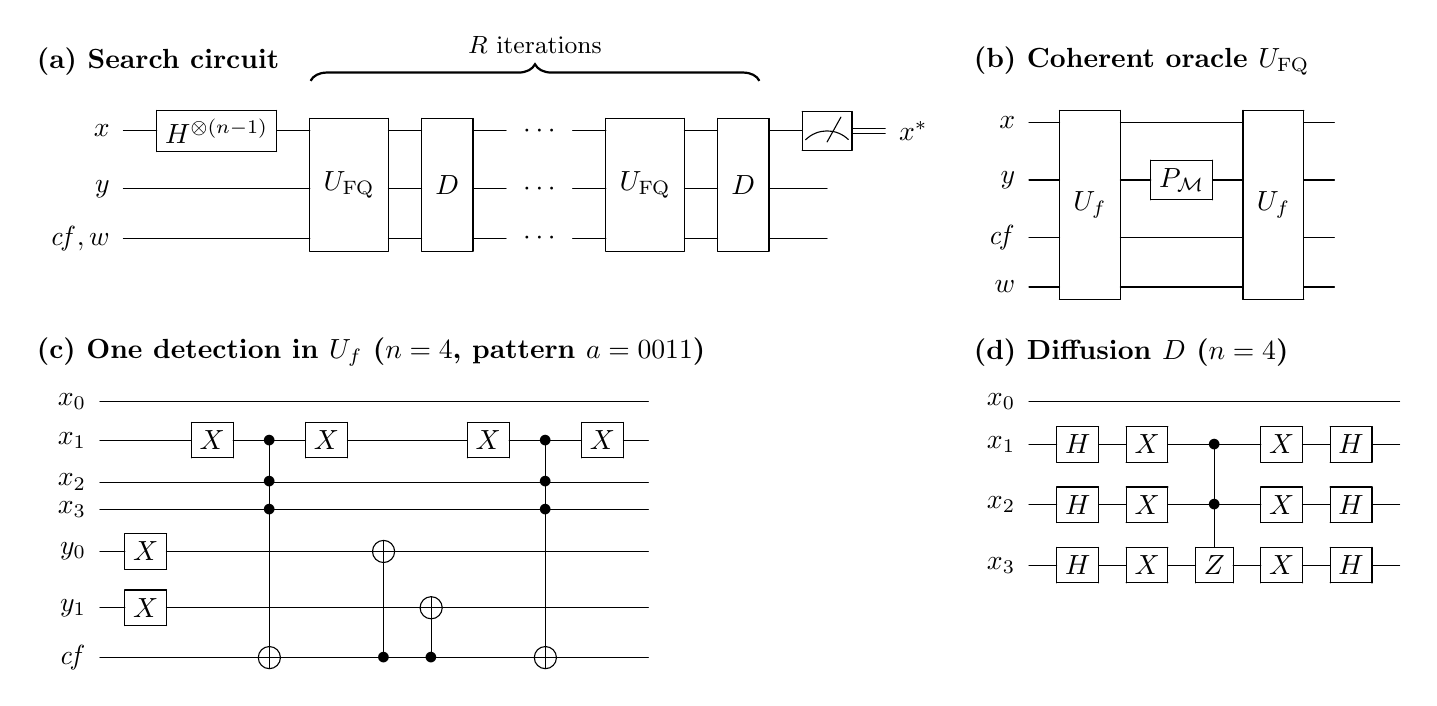
\begin{tikzpicture}
\node[anchor=south west] at (0,6.0) {\textbf{(a) Search circuit}};
\node[anchor=north west] at (1.1,5.8) {
  \Qcircuit @C=1.2em @R=0.9em {
    \lstick{x} & \gate{H^{\otimes(n-1)}} & \multigate{2}{U_{\mathrm{FQ}}} & \multigate{2}{D} & \qw & \cdots & & \multigate{2}{U_{\mathrm{FQ}}} & \multigate{2}{D} & \meter & \rstick{x^{*}}\cw \\
    \lstick{y} & \qw & \ghost{U_{\mathrm{FQ}}} & \ghost{D} & \qw & \cdots & & \ghost{U_{\mathrm{FQ}}} & \ghost{D} & \qw & \\
    \lstick{\mathit{cf},w} & \qw & \ghost{U_{\mathrm{FQ}}} & \ghost{D} & \qw & \cdots & & \ghost{U_{\mathrm{FQ}}} & \ghost{D} & \qw &
  }
};
\draw[thick, decorate, decoration={brace, amplitude=6pt}]
  (3.6,6.05) -- (9.3,6.05) node[midway, above=6pt] {\small $R$ iterations};
\node[anchor=south west] at (11.9,6.0) {\textbf{(b) Coherent oracle $U_{\mathrm{FQ}}$}};
\node[anchor=north west] at (12.6,5.8) {
  \Qcircuit @C=1.1em @R=0.9em {
    \lstick{x} & \multigate{3}{U_f} & \qw & \multigate{3}{U_f} & \qw \\
    \lstick{y} & \ghost{U_f} & \gate{P_{\mathcal{M}}} & \ghost{U_f} & \qw \\
    \lstick{\mathit{cf}} & \ghost{U_f} & \qw & \ghost{U_f} & \qw \\
    \lstick{w} & \ghost{U_f} & \qw & \ghost{U_f} & \qw
  }
};
\node[anchor=south west] at (0,2.3) {\textbf{(c) One detection in $U_f$ ($n=4$, pattern $a=0011$)}};
\node[anchor=north west] at (0.8,2.1) {
  \Qcircuit @C=0.9em @R=0.75em {
    \lstick{x_0} & \qw & \qw & \qw & \qw & \qw & \qw & \qw & \qw & \qw & \qw \\
    \lstick{x_1} & \qw & \gate{X} & \ctrl{5} & \gate{X} & \qw & \qw & \gate{X} & \ctrl{5} & \gate{X} & \qw \\
    \lstick{x_2} & \qw & \qw & \ctrl{4} & \qw & \qw & \qw & \qw & \ctrl{4} & \qw & \qw \\
    \lstick{x_3} & \qw & \qw & \ctrl{3} & \qw & \qw & \qw & \qw & \ctrl{3} & \qw & \qw \\
    \lstick{y_0} & \gate{X} & \qw & \qw & \qw & \targ & \qw & \qw & \qw & \qw & \qw \\
    \lstick{y_1} & \gate{X} & \qw & \qw & \qw & \qw & \targ & \qw & \qw & \qw & \qw \\
    \lstick{\mathit{cf}} & \qw & \qw & \targ & \qw & \ctrl{-2} & \ctrl{-1} & \qw & \targ & \qw & \qw
  }
};
\node[anchor=south west] at (11.9,2.3) {\textbf{(d) Diffusion $D$ ($n=4$)}};
\node[anchor=north west] at (12.6,2.1) {
  \Qcircuit @C=1.0em @R=0.9em {
    \lstick{x_0} & \qw & \qw & \qw & \qw & \qw & \qw \\
    \lstick{x_1} & \gate{H} & \gate{X} & \ctrl{2} & \gate{X} & \gate{H} & \qw \\
    \lstick{x_2} & \gate{H} & \gate{X} & \ctrl{1} & \gate{X} & \gate{H} & \qw \\
    \lstick{x_3} & \gate{H} & \gate{X} & \gate{Z} & \gate{X} & \gate{H} & \qw
  }
};
\end{tikzpicture}}
\caption{Coherent-oracle search for family $\famE$, drawn for the four-bit
benchmark ($s=1010$, representative bit $b=0$, so $x_b=x_0$). (a) All registers
start in $\ket{0}$: $x$ and $y$ with $n$ qubits each, $\mathit{cf}$ with one, and
$w$ with $n-2$. State preparation applies $H$ to every input qubit except $x_b$,
so the register holds the $2^{n-1}$ canonical representatives. $R$ rounds of the
oracle and diffusion follow, and $x$ is measured once at the end, giving $x^{*}$. (b) The oracle
computes $f$ into $y$, flips the sign of outputs in $\mathcal{M}$, and computes
$f$ again to clear $y$ (the work register $w$ serves the decompositions). (c)
Detection of the canonical pattern $a=0011$. The first $X$ gates write the
default $\delta=1111$ (wires $y_2,y_3$ omitted). The $X$ gate on $x_1$ selects
the zero of $a$, and the multi-controlled $X$ raises $\mathit{cf}$. CNOTs then
add $\delta\oplus o=1100$ to $y$, and the detection repeats to clear
$\mathit{cf}$. The bit $x_b$ is never a control. (d) Diffusion acts on the $n-1$
search qubits only. No measurement occurs before the final readout.}
\label{fig:circuit}
\end{figure*}

The compile-time (CT) oracle is a sequence of $k$ multi-controlled $Z$ gates on
the search qubits, one per marked input; such a gate flips the sign of the state
in which all its qubits are 1. $X$ gates (bit flips) on either side select the
zeros of that input. The oracle is cheap when $k$ is small, but the compiler
must know every marked input. Marked inputs that form a cube, a set of inputs
that agree on fixed bits, share one gate on those bits. By default the selection
pass builds CT as a cover of disjoint cubes: two cubes that differ in one fixed
bit merge, until no pair does. The two marked inputs of our benchmark instances
differ in two bits and do not merge, so there the cover equals the
one-gate-per-input form. Stronger syntheses (Section~\ref{sec:cost}) only make CT
cheaper, so the ratios we report where CT already wins are lower bounds
(Section~\ref{S-sec:thr}).

The coherent oracle is $U_{\mathrm{FQ}}=U_f^{\dagger}\,P_{\mathcal{M}}\,U_f$.
Here $U_f\ket{x,y}=\ket{x,y\oplus f(x)}$ adds $f(x)$ to an output register $y$,
and $P_{\mathcal{M}}\ket{y}=(-1)^{g(y)}\ket{y}$ flips the sign of the outputs
that pass the membership test $g(y)=[y\in\mathcal{M}]$. The design therefore needs
a circuit for $f$ and one for $g$, but no list of marked inputs. $U_f$ must act correctly only
on canonical inputs $x\in\Xo$, since no other input enters the search register.
For family $\famE$ the oracle uses an input register $x$ ($n$ qubits), an output
register $y$ ($n$ qubits), a coset flag $\mathit{cf}$ (one qubit), and a work
register $w$ ($n-2$ qubits), as in Fig.~\ref{fig:circuit}. Its three parts are as
follows.
\begin{itemize}
\item $U_f$ writes $\delta$ into $y$ with $X$ gates. For each exceptional coset,
it detects $a_i$ with a multi-controlled $X$ from the $n-1$ bits other than
$x_b$ onto $\mathit{cf}$. It then adds $\delta\oplus o_i$ to $y$ with CNOTs
controlled by $\mathit{cf}$ and repeats the detection to clear $\mathit{cf}$.
For family $\famL$, $U_f$ is the CNOT network that adds $Lx$ to $y$; on $\Xo$
the column of $L$ for bit $b$ is not needed, and no flag is used. For family
$\famN$ it adds the $t$ products with Toffoli gates.
\item $P_{\mathcal{M}}$ implements $g$ for an explicit set of outputs: for each
$m\in\mathcal{M}$, a multi-controlled $Z$ on $y$ that selects $m$ with $X$
gates. Any other circuit for $g$, such as a comparator, fits the same slot.
\item $U_f^{\dagger}$ clears $y$. Because $U_f$ adds $f(x)$ to $y$ modulo 2,
applying it twice gives the identity, so $U_f^{\dagger}=U_f$.
\end{itemize}
Algorithm~\ref{S-alg:fqdoa} gives the full procedure.

The FQ-DOA design gives one coherent oracle per family: we call those of families
$\famL$ and $\famN$ Lin and Quad, and reach that of family $\famE$, called D3, from
a design variant D0 in four compilation steps. D0 evaluates $f$ on all $2^n$ inputs. It detects
both members of every exceptional coset with $n$ controls and sets a membership
flag, which an extra qubit in $\ket{-}$ turns into a sign flip before the flag is
cleared; D0 uses $3n+1$ qubits in total. D1 detects only the canonical member and
drops $x_b$ as a control (steps O1 and O2). D2 replaces the flag and the extra
qubit by the multi-controlled $Z$ gates of $P_{\mathcal{M}}$ (step O3), which
saves two qubits. D3 uses relative-phase Toffolis inside each multi-controlled
gate (step O4, Section~\ref{sec:cost}). All variants share state preparation,
diffusion, and the decomposition code, and each step keeps the circuit correct on
$\Xo$.


\subsection{Correctness of the Coherent Oracle}
\label{sec:correctness}

We now show that the coherent oracle flips the sign of exactly the marked
canonical inputs and restores every auxiliary register. Write $\ket{x,y}$ for
the input and output registers and omit $\mathit{cf}$ and $w$ when they hold
$\ket{0}$.

\begin{lemma}\label{lem:uf}
For every $x\in\Xo$ and every $y$, $U_f\ket{x,y}=\ket{x,y\oplus f(x)}$, and
$\mathit{cf}$ and $w$ return to $\ket{0}$.
\end{lemma}
\begin{IEEEproof}
For family $\famL$ the CNOT network adds $Lx$ to $y$, and $Lx=f(x)$ on $\Xo$.
For family $\famN$ the CNOTs add $x$ and the Toffoli gates add the products, so
$y$ gains $F(x)=f(x)$ on $\Xo$; neither network uses $\mathit{cf}$ or $w$. For
family $\famE$, the $X$ gates add $\delta$ to $y$, and the detection of $a_i$
fires when $x$ agrees with $a_i$ on every bit except $b$. On $\Xo$ both $x_b$
and $(a_i)_b$ are 0, so it fires exactly when $x=a_i$, and at most one detection
fires because the $a_i$ are distinct. The CNOTs then add $\delta\oplus o_i$ if
$x=a_i$, so $y$ ends at $y\oplus o_i=y\oplus f(x)$, and otherwise at
$y\oplus\delta=y\oplus f(x)$. Each detection runs twice with the same controls,
which clears $\mathit{cf}$. Inside each detection, the ladder gates of the
decomposition are undone in reverse order, which clears $w$ and cancels their
relative phases~\cite{maslov2016advantages}.
\end{IEEEproof}

\begin{lemma}\label{lem:pm}
$P_{\mathcal{M}}\ket{y}=(-1)^{[y\in\mathcal{M}]}\ket{y}$.
\end{lemma}
\begin{IEEEproof}
The multi-controlled $Z$ for $m$ flips the sign of $\ket{y}$ exactly when
$y=m$. The elements of $\mathcal{M}$ are distinct, so at most one gate fires.
\end{IEEEproof}

\begin{proposition}\label{prop:oracle}
For every $x\in\Xo$, $U_{\mathrm{FQ}}\ket{x,0}=(-1)^{[f(x)\in\mathcal{M}]}\ket{x,0}$.
\end{proposition}
\begin{IEEEproof}
By Lemma~\ref{lem:uf}, $U_f$ gives $\ket{x,f(x)}$. By Lemma~\ref{lem:pm},
$P_{\mathcal{M}}$ multiplies it by $(-1)^{[f(x)\in\mathcal{M}]}$. By
Lemma~\ref{lem:uf} again, $U_f^{\dagger}=U_f$ gives
$\ket{x,f(x)\oplus f(x)}=\ket{x,0}$.
\end{IEEEproof}

\begin{proposition}\label{prop:success}
After $R$ iterations, the probability of measuring a marked input is
$\sin^2((2R+1)\theta)$, where $\sin^2\theta=k/2^{n-1}$.
\end{proposition}
\begin{IEEEproof}
State preparation gives the uniform superposition over $\Xo$. No gate changes
$x_b$, so the state stays in the span of $\Xo$. On that span,
Proposition~\ref{prop:oracle} makes $U_{\mathrm{FQ}}$ the standard phase oracle,
and diffusion reflects about the uniform state. The claim is then the usual
analysis of Grover's algorithm with $k$ marked items among
$2^{n-1}$~\cite{boyer1998tight}.
\end{IEEEproof}

Proposition~\ref{prop:success} also holds for the compile-time oracle, whose
gates mark the $k$ inputs directly. We checked Proposition~\ref{prop:oracle}
numerically by simulating $U_{\mathrm{FQ}}$ on every canonical input for $n=4$
and $n=6$, for all three families. The largest deviation from the stated action was
\val{cor.oracle_err_all}.

\begin{proposition}\label{prop:restriction}
Searching all $2^n$ inputs, with every $x$ such that $f(x)\in\mathcal{M}$
marked, needs the same number of iterations and reaches the same success
probability as searching $\Xo$.
\end{proposition}
\begin{IEEEproof}
Since $f(x)=f(x\oplus s)$, marked inputs come in pairs, so the full space holds
$2k$ of them. Hence $\sin^2\theta'=2k/2^n=k/2^{n-1}=\sin^2\theta$, and
Proposition~\ref{prop:success} gives the same iteration count and success
probability.
\end{IEEEproof}

The restriction to canonical representatives therefore saves no Grover
iterations. Its benefit is structural: the search register loses one qubit, and
every multi-controlled gate loses one control.

\subsection{Cost Model and the Cost of Coherence}
\label{sec:cost}

We decompose each multi-controlled $X$ with $n_c\ge 3$ controls into a chain of
$2n_c-3$ Toffoli gates that uses $n_c-2$ work
qubits~\cite{barenco1995elementary}. The $2n_c-4$ ladder Toffolis come in
compute and uncompute pairs, so we implement them as relative-phase Toffolis
with three CNOTs and four T gates~\cite{maslov2016advantages}. Only the Toffoli
that flips the target stays a full Toffoli, with six CNOTs and seven T
gates~\cite{shende2009cnot,amy2013meet}. A multi-controlled $X$ with $n_c$
controls therefore uses $8n_c-9$ T gates in this decomposition. The formula also
holds for $n_c=2$. The next result gives the cost of both oracles for any $f$.

\begin{proposition}[Cost of coherence]\label{prop:coherence}
Let $n\ge 4$, and let $U_f$ use $T_f$ T gates. Per iteration, the coherent oracle and diffusion use
$2T_f+|\mathcal{M}|(8n-17)+(8n-25)$ T gates, and the compile-time oracle with
one gate per marked input and diffusion use $(k+1)(8n-25)$. If $f$ is two-to-one
and every element of
$\mathcal{M}$ has a preimage, then $k=|\mathcal{M}|$, and the coherent oracle
needs exactly $2T_f+8|\mathcal{M}|$ more T gates per iteration.
\end{proposition}
\begin{IEEEproof}
$P_{\mathcal{M}}$ holds $|\mathcal{M}|$ multi-controlled $Z$ gates on $y$, each a
multi-controlled $X$ with $n-1$ controls and $8n-17$ T gates. Diffusion holds
one with $n-2$ controls and $8n-25$ T gates, and $U_f$ runs twice. The
compile-time oracle holds $k$ gates with $n-2$ controls. Under the last two
conditions, each element of $\mathcal{M}$ has exactly two preimages, which form one coset with one
canonical member, so $k=|\mathcal{M}|$. Subtracting gives
$2T_f+|\mathcal{M}|\,[(8n-17)-(8n-25)]=2T_f+8|\mathcal{M}|$.
\end{IEEEproof}

If $g$ is given as another circuit with $T_g$ T gates, $T_g$ replaces
$|\mathcal{M}|(8n-17)$ in both statements. Per iteration, the coherent oracle
therefore needs fewer T gates exactly when $2T_f+T_g$ is below the T-count of
the compile-time marking circuit, whichever synthesis produced it. The price of
coherence is thus the two
evaluations of $f$ plus the difference between testing outputs and listing
inputs.

\textit{Threshold tests.} A test can mark many outputs with few gates. For
$\mathcal{M}=\{y:y<\tau\}$, $P_{\mathcal{M}}$ needs one multi-controlled $Z$ per
1 bit of $\tau$, on that bit and the bits above it. These gates mark disjoint
sets whose union is $\mathcal{M}$, so Lemma~\ref{lem:pm} holds, and
$T_g$ does not grow with $|\mathcal{M}|$. A compiler can also compress the list, so we compare
three compile-time syntheses: a cube cover, the cheapest fixed-polarity
Reed--Muller form, and a cover by affine subspaces, an XOR-AND-XOR
form~\cite{bernasconi2023xor} (Section~\ref{S-sec:thr}). We add a synthetic family
$\famR$, the quadratic layer of family $\famN$ followed by the linear layer of
family $\famL$, shaped like one round of a substitution--permutation cipher but
not a real cipher, with $T_f=7t$. Lemma~\ref{lem:uf} extends to it
(Section~\ref{S-sec:thr}), and Section~\ref{sec:threshold} reports the outcome.

For family $\famE$, $U_f$ holds $2c$ multi-controlled $X$ gates with $n-1$
controls, so $T_f=2c(8n-17)$. Over $R$ iterations the Toffoli and T counts are
\begin{equation}
\begin{aligned}
N^{\mathrm{FQ}}_{\mathrm{Tof}} &= R\,[(4c+|\mathcal{M}|)(2n-5)+(2n-7)],\\
N^{\mathrm{FQ}}_{T} &= R\,[(4c+|\mathcal{M}|)(8n-17)+(8n-25)],
\end{aligned}
\label{eq:costfq}
\end{equation}
and the compile-time oracle needs
\begin{equation}
N^{\mathrm{CT}}_{\mathrm{Tof}} = R\,(k+1)(2n-7),\qquad
N^{\mathrm{CT}}_{T} = R\,(k+1)(8n-25).
\label{eq:costct}
\end{equation}

\begin{proposition}\label{prop:cheaper}
For family $\famE$ with $\delta\notin\mathcal{M}$ and at least one marked input, $k\le c$ and
$N^{\mathrm{FQ}}_{\mathrm{Tof}}/N^{\mathrm{CT}}_{\mathrm{Tof}} >
(4c+|\mathcal{M}|+1)/(c+1) \ge 3$. The same bound holds for T gates.
\end{proposition}
\begin{IEEEproof}
If $\delta\notin\mathcal{M}$, only exceptional inputs can be marked. Each
exceptional coset has one canonical member, so $k\le c$. Since $2n-5>2n-7>0$
for $n\ge 4$, dividing \eqref{eq:costfq} by \eqref{eq:costct} gives a ratio
greater than $(4c+|\mathcal{M}|+1)/(k+1)\ge(4c+|\mathcal{M}|+1)/(c+1)$. A
marked input needs $|\mathcal{M}|\ge 1$ and $c\ge k\ge 1$, so the bound is at
least $(4c+2)/(c+1)\ge 3$. The T-gate case follows in the same way from
$8n-17>8n-25>0$.
\end{IEEEproof}

A cube cover can only lower $N^{\mathrm{CT}}$, so the bound holds against it as
well. When $\delta\in\mathcal{M}$, all but at most $c$ canonical inputs are
marked, and a random guess succeeds with probability at least $1-c/2^{n-1}$. In
D3, the two evaluations of $f$ take \val{blk.D3.n4.uf_share} of the T gates of an
iteration at $n=4$ and \val{blk.D3.n14.uf_share} at $n=14$
(Table~\ref{S-tab:blocks}).

For family $\famL$, $T_f=0$, and $f$ is two-to-one. When its image contains
$\mathcal{M}$, Proposition~\ref{prop:coherence} gives the coherent oracle only
$8|\mathcal{M}|$ more T gates per iteration, and the T-count ratio
$[|\mathcal{M}|(8n-17)+(8n-25)]/[(|\mathcal{M}|+1)(8n-25)]$ tends to one as $n$
grows. Its extra cost moves to the CNOT network: two evaluations add twice the
number of ones in $L$ outside column $b$, up to $2n(n-1)$ CNOTs per iteration.
For family $\famN$, $T_f=7t$, so in the same case the coherent oracle adds
$14t+8|\mathcal{M}|$ T gates per iteration; $t$ moves the cost between that of family $\famL$ at $t=0$
and that of costly functions such as family $\famE$.

\textit{Other decompositions.} If a gate with $n_c$ controls costs $T(n_c)$ T
gates, the extra cost in Proposition~\ref{prop:coherence} becomes
$2T_f+|\mathcal{M}|\,[T(n-1)-T(n-2)]$, and Proposition~\ref{prop:cheaper} holds
for every $T$ that grows with $n_c$. Logical AND gates undone by
measurement~\cite{gidney2018halving}, $T(n_c)=4(n_c-1)$, also clear each flag
for free, so $U_f$ holds $c$ gates and the bound falls to
$(2c+|\mathcal{M}|+1)/(c+1)\ge 2$. Measurement-based
uncomputation~\cite{luongo2025measurement} leaves one evaluation of $f$ for
families $\famL$ and $\famN$ (Section~\ref{S-sec:other}). Both measure in every
iteration, which our hardware runs avoid.

\begin{proposition}[Cost of listing]\label{prop:listing}
For family $\famE$ with $\delta\notin\mathcal{M}$, the marked canonical inputs
are the $a_i$ with $o_i\in\mathcal{M}$, found with $O(cn)$ bit operations. For
family $\famL$, they are the vectors $L^{-1}m$ for $m\in\mathcal{M}$ whose bit $b$
is 0, found with $O(n^3+|\mathcal{M}|\,n^2)$ bit operations. For family
$\famN$, they are found with $O(|\mathcal{M}|(n+t))$ bit operations.
\end{proposition}
\begin{IEEEproof}
For family $\famE$, inputs outside the exceptional cosets map to
$\delta\notin\mathcal{M}$, so only the canonical members $a_i$ can be marked.
Checking the $c$ outputs $o_i$ against a hash set of $\mathcal{M}$ costs $O(cn)$.
For family $\famL$, the value $x\oplus x_bs$ always has bit $b$ equal to 0, so
$f(x)=m$ has a solution exactly when $L^{-1}m$ has bit $b$ equal to 0, and that
vector is the canonical solution. Inverting $L$ by Gaussian elimination costs
$O(n^3)$, and each product $L^{-1}m$ costs $O(n^2)$. For family $\famN$, $F$ is
triangular, so $F(z)=m$ is solved bit by bit in increasing order. Each bit adds
the products of bits already found, which costs $O(n+t)$ per element of
$\mathcal{M}$, and the solution is kept if its bit $b$ is 0.
\end{IEEEproof}

If $f$ is available only as a black box, no such shortcut exists. Random sampling
of canonical inputs then needs $(2^{n-1}+1)/(k+1)$ evaluations of $f$ on average,
the mean position of the first marked input in a random order. The
compile-time oracle can be built only after a classical search that
already solves the problem.

The coherent oracle allocates $3n-1$ qubits for family $\famE$ and $3n-2$ for
families $\famL$ and $\famN$, which need no flag. The compile-time oracle needs $n$ input qubits and $n-4$ work qubits for $n\ge 5$.

\subsection{Cost of Finding the Period and of the Whole Pipeline}
\label{sec:simon}

The period comes from Simon's algorithm. Each sample applies $H^{\otimes n}$,
$U_f$ on all inputs, and $H^{\otimes n}$ again, and returns a $y$ with $y\cdot
s=0$, where $y\cdot s=\bigoplus_i y_is_i$. Once the samples span the
$(n-1)$-dimensional space orthogonal to $s$, the period is determined. This takes $O(n)$ samples when $f(x)=f(y)$ holds only
for $y\in\{x,x\oplus s\}$~\cite{simon1994power}, as it does for families $\famL$
and $\famN$. Family $\famE$ breaks that condition, since all inputs outside the
exceptional cosets share one output.

\begin{proposition}\label{prop:simon}
Let $f$ be in family $\famE$ with $c$ exceptional cosets whose outputs are
distinct and differ from $\delta$. Every Simon sample $y\neq 0$ then has
probability at most $4c(c+1)/4^n$, a sample is nonzero with probability less
than $c(c+1)2^{1-n}$, and recovering $s$ needs more than $(n-1)2^{n-1}/(c(c+1))$
samples in expectation.
\end{proposition}
\begin{IEEEproof}
With $N=2^n$, a sample equals $y$ with probability $\sum_z
|N^{-1}\sum_{x:f(x)=z}(-1)^{x\cdot y}|^2$. If $y\cdot s=1$, the two members of
every coset cancel. Take $y\neq 0$ with $y\cdot s=0$ and write
$\chi_i=(-1)^{a_i\cdot y}$. Each exceptional output collects one coset, whose sum
is $2\chi_i$, and contributes $4/N^2$. The default output collects all other
inputs, and since the sum over all inputs is 0, its sum is $-2\sum_i\chi_i$, of
magnitude at most $2c$. Hence $y$ has probability at most $(4c+4c^2)/N^2$, and
since fewer than $2^{n-1}$ such $y$ exist, a sample is nonzero with probability
less than $c(c+1)2^{1-n}$. A zero sample carries no information, and spanning a
space of dimension $n-1$ needs $n-1$ nonzero samples.
\end{IEEEproof}

The bound is exponential in $n$ for any fixed number of exceptions, so the
$O(n)$ bound of Kaplan et al.~\cite{kaplan2016breaking} does not apply. In their
terms, the collision probability $\varepsilon=\max_{u\notin\{0,s\}}\Pr_x[f(x\oplus u)=f(x)]$ is \val{simon.n4.eps} at $n=4$
and \val{simon.n14.eps} at $n=14$ for our family $\famE$ benchmark, and zero for
families $\famL$ and $\famN$. In Table~\ref{S-tab:simon}, the mean number of
samples for family $\famE$ grows from \val{simon.n4.runs} at $n=4$ to
\val{simon.n14.runs} at $n=14$, above the bound of \val{simon.n14.bound}. For
families $\famL$ and $\famN$ the samples are uniform on the space orthogonal to
$s$, and fewer than $n+1$ suffice on average.

\textit{The whole pipeline.} A coherent search that must first find the period
costs, in T gates,
\begin{equation}
T_{\mathrm{pipe}} = S\,T_S + R\,T_{\mathrm{it}},
\label{eq:pipeline}
\end{equation}
where $S$ is the expected number of Simon samples, $T_S$ the T-count of one
sample, and $T_{\mathrm{it}}$ that of one search iteration. A compile-time search
pays instead the classical listing cost of Proposition~\ref{prop:listing} and
$R\,T^{\mathrm{CT}}_{\mathrm{it}}$, with $T^{\mathrm{CT}}_{\mathrm{it}}$ the
T-count of one of its iterations. For family $\famE$ the Simon stage costs
\val{pipe.E_ratio_min} to \val{pipe.E_ratio_max} times the search
(Table~\ref{S-tab:simon}), so the period-first pipeline is not worth running. For
family $\famN$ the Simon stage costs at most \val{pipe.N_share_max} of the total,
and for family $\famL$ it needs no T gates. In the experiments we take $s$ from
the function description, as a compile-time design would.
\subsection{Oracle Selection Pass}
\label{sec:select}

We turn the comparison into a compiler pass (Algorithm~\ref{alg:select}). Its
inputs are a period-restricted search problem, a classical budget $B$, and a
target. It first estimates the cost of listing the marked inputs from the
function description (Proposition~\ref{prop:listing}); a black box allows only
random sampling. If listing fits the budget, both designs are candidates, and
otherwise only the coherent oracle is. The pass selects among the representations
it is given; a stronger synthesis enters it as one more candidate. For an
error-corrected target the pass
costs each candidate with Proposition~\ref{prop:coherence} and keeps the one
with fewer T gates. For a current device it routes every candidate for every
iteration count $R'\le R$ and predicts its success with a calibrated heuristic
model of the backend.
\begin{equation}
P=\Phi\,P_0+(1-\Phi)\,k/2^n,\qquad \Phi=(1-p_{\mathrm{eff}})^G.
\label{eq:survival}
\end{equation}
In Eq.~\eqref{eq:survival}, $P_0$ is the noiseless success, $G$ the routed
two-qubit count, $p_{\mathrm{eff}}$ one error rate per routed two-qubit gate,
fitted to a single calibration circuit on the target, and $\Phi$ the probability
that no error occurs. The model lumps every error source into
$p_{\mathrm{eff}}$, in the spirit of the digital error model
of~\cite{arute2019quantum}, and a failure sends the register to the chance level
$k/2^n$, that of a fully mixed register.
We use it as a ranking heuristic: the pass needs the order of the candidates, not
their exact success.
The pass returns the design and $R'$ with the highest prediction and warns when
that prediction does not exceed the no-search level $k/2^{n-1}$, the success of
measuring the prepared state without any search. As a Qiskit transpiler
pass it takes at most \val{po.ec.max}~s for an error-corrected target up to
$n=14$, and up to \val{po.dev.ratio.max} times one routing of its output for a
device (Section~\ref{S-sec:decisions}).

\begin{algorithm}[!t]
\caption{Oracle selection pass.}
\label{alg:select}
\small
\KwIn{$f$ as a circuit $U_f$ or a structure; marked set $\mathcal{M}$;
classical budget $B$; target: error-corrected, or a device with $p_{\mathrm{eff}}$.}
\KwOut{An oracle circuit and a cost report.}
Estimate the listing cost $C_{\mathrm{list}}$ (Proposition~\ref{prop:listing})\;
$\mathcal{D}\gets\{\text{coherent}\}$; \lIf{$C_{\mathrm{list}}\le B$}{$\mathcal{D}\gets \mathcal{D}\cup\{\text{compile-time}\}$}
\eIf{the target is error-corrected}{
  \Return the design in $\mathcal{D}$ with fewer T gates, breaking ties by qubits\;}{
  \ForEach{design in $\mathcal{D}$ and each $R'\le R$}{
    Route the circuit and count its two-qubit gates $G$\;
    Predict $P$ with Eq.~\eqref{eq:survival}\;}
  \Return the pair with the highest $P$, and warn if $P\le k/2^{n-1}$\;}
\end{algorithm}

% ============================================================
\section{Experiments}
\label{sec:experiments}

This section describes the setup, then reports the cost of the oracles and how
it varies with the function, the ablation of the compilation steps, the
comparison under noise, the hardware runs, and the validation of the selection
pass.

\subsection{Setup}
\label{sec:setup}

\textit{Metrics.} We measure three kinds of quantity. Logical cost, in Toffoli
gates, T gates, and T-depth, follows from the circuit alone and dominates time
and space on an error-corrected machine, where every T gate consumes a costly
resource state~\cite{amy2013meet,babbush2018encoding}. Compiled cost counts
two-qubit gates and depth after transpilation, the compilation of a circuit to
the gates and connectivity of a device. It predicts how much noise a circuit
collects on current hardware: on the Heron~r2 model the median two-qubit error
is \val{dev.cz}, about \val{dev.cz_over_sx} times the single-qubit error. Success
is the probability that the measured $x$ is a marked canonical input. Measuring
the prepared state without any search gives $k/2^{n-1}$, which is
\val{ref.nosearch.n4} at $n=4$ and \val{ref.nosearch.n6} at $n=6$; we call this
the no-search level and success above it amplification. A fully mixed register
gives $k/2^n$, which is \val{ref.floor.n4} and \val{ref.floor.n6}; we call this
the chance level.

\textit{Benchmark families.} For even $n$ we set $s=(10)^{n/2}$, so $b=0$. For
family $\famE$, $\delta=1^n$, $\mathcal{M}=\{0^n,0^{n-2}11\}$, and the exceptional
cosets are $\{0^n,s\}\mapsto 0^n$ and $\{0^{n-2}11,\,0^{n-2}11\oplus s\}\mapsto
0^{n-2}11$, so $c=2$ and $|\mathcal{M}|=k=2$. For family $\famL$ we draw $L$ at
random with a fixed seed per $n$. For family $\famN$ we draw $t=n$ products with a
fixed seed, capped by the number admissible, so $t=1$ at $n=4$. In both we mark
the images of the same two canonical inputs, so $k=2$ and the compile-time oracle
is the same for all three families. The families were fixed in advance and not
tuned.

\textit{Designs.} We compare the four variants of family $\famE$ (D0 to D3), and
the coherent oracles for families $\famL$ (Lin) and $\famN$ (Quad), with the
compile-time oracle (CT).
All are built by the same code, with the same decompositions and the same $R$.
CT is the cube cover of Section~\ref{sec:styles}, which for these instances
places one gate per marked input.

\textit{Simulation.} We use Qiskit \val{meta.qiskit}~\cite{javadiabhari2024quantum}
and its simulator Qiskit Aer \val{meta.qiskit_aer}. We transpile to the gate set
$\{cx,id,rz,sx,x\}$: the CNOT ($cx$), the identity ($id$), rotations about the $Z$
axis ($rz$), the square root of $X$ ($sx$), and the Pauli $X$ gate ($x$). We use
Qiskit's optimization level 1 (of 0 to 3) with all-to-all connectivity, so any
two qubits may interact. The noise model applies a
depolarizing channel of strength $p$ after every one- and two-qubit gate: with
probability $p$ it replaces the state of the qubits the gate acts on by the fully
mixed state. It includes $rz$, which IBM hardware applies without error by
adjusting later pulses, so the model is pessimistic, and it leaves measurement
noiseless. At $n=4$ we compute exact probabilities from the density matrix. At
$n=6$ the density matrices of the coherent oracles are too large, and we sample
\val{nz6.shots} noisy trajectories per point, Monte Carlo runs with random
errors, and report 95\% Wilson intervals for the resulting proportions.

\textit{Routing.} We transpile to the coupling map, the graph of qubit pairs
that can interact, and the native gates $\{cz,id,rz,sx,x\}$ of the 156-qubit
Heron~r2 model FakeFez from qiskit-ibm-runtime \val{meta.qiskit_ibm_runtime},
where $cz$ is the controlled-$Z$ gate. We use optimization level 3 and
\val{route.D3.n4.seeds} random seeds of the transpiler at $n=4$ and
\val{route.D3.n6.seeds} at $n=6$, 8, and 10. We compare against the same optimization level and gate set without a
coupling map.

\textit{Hardware.} We ran through IBM's SamplerV2 interface, which returns
measurement counts, with \val{hw.shots} shots, or repetitions, per circuit and
run. On \val{hw.A.date} (\val{hw.A.start} to \val{hw.A.end} UTC) D3 ran alone on
\texttt{ibm\_fez}, in \val{hw.runs_word} jobs per size. On \val{hw.B.date}
\val{hw.B.njobs} jobs each held all \val{hw.B.ncirc} circuits of
Table~\ref{tab:matched}, so the designs of a job share one calibration; they ran
on \texttt{ibm\_fez} (\val{hw.B.start} to \val{hw.B.end} UTC) and on
\texttt{ibm\_marrakesh} (\val{hw.C.start} to \val{hw.C.end} UTC). We transpiled at optimization
level 3 against the calibration of the day, the error rates and coherence times
that IBM measures for each qubit and coupler. We used no mid-circuit measurement
and no error mitigation, the post-processing that corrects results for noise.
Section~\ref{S-sec:hwrec} lists every job, its success, and the
calibration in force. We report the mean
over runs, the sample standard deviation, and a 95\% interval with the
Student-$t$ quantile \val{hw.tq} for four degrees of freedom.

\textit{Device models.} To test the selection pass beyond one device, we use the
noise models of five IBM devices from qiskit-ibm-runtime, built from their
published calibrations. They span three processor generations: FakeFez and
FakeMarrakesh (Heron~r2), FakeTorino (Heron~r1), and FakeSherbrooke and
FakeBrisbane (Eagle~r3). On each we route every candidate with transpiler
seed 0, and with seeds 1 and 2 to test robustness, and
simulate it with the device's noise model, with \val{fake.shots} shots, or
\val{fake.shots_wide} for circuits wider than 16 qubits. The budget $B$ admits
listing from the function description but not black-box enumeration, so each
decision is made with and without listing.

\subsection{Cost of the Oracles and How It Varies}
\label{sec:resources}

Table~\ref{tab:resources} gives the cost of the coherent oracles relative to CT
from $n=4$ to $n=14$, and Table~\ref{S-tab:resources} and Fig.~\ref{S-fig:scaling}
give the absolute counts. For family $\famE$, D3 needs \val{res.tratio_min}
to \val{res.tratio_max} times the T gates of CT, in line with
Proposition~\ref{prop:cheaper}. For family $\famL$ the ratio falls from
\val{res.n4.tratio_LIN} at $n=4$ to \val{res.n14.tratio_LIN} at $n=14$. For
family $\famN$ it lies between the two, at \val{res.n14.tratio_Q} at $n=14$, as
Proposition~\ref{prop:coherence} predicts with $T_f=7t$.

The two-qubit counts tell a different story. After transpilation, D3 needs
\val{res.n2q_ratio_min} to \val{res.n2q_ratio_max} times the two-qubit gates of
CT. The CNOT network of family $\famL$ grows with $n^2$, so Lin needs
\val{res.n2q_ratio_LIN_min} to \val{res.n2q_ratio_LIN_max} times as many as CT,
and at $n=14$ it needs more than D3. The cost of coherence therefore depends on
the metric. The T-count, which dominates error-corrected cost, favors compact
circuits, while the two-qubit count, which limits current hardware, penalizes
dense CNOT networks. Fig.~\ref{S-fig:sensitivity} shows how the price of
coherence moves with the number of exceptions, products, and ones in $L$.

The T-depth, which sets the running time of an error-corrected machine when many
T gates can run at once, ranks the designs as the T-count does at every $n$
(Table~\ref{S-tab:resources}). D3 needs \val{res.tdratio_min} to
\val{res.tdratio_max} times the T-depth of CT.

\begin{table}[!t]
\caption{Cost of the coherent oracles (D3, Lin, Quad for families $\famE$,
$\famL$, $\famN$) relative to the compile-time oracle (CT) for the whole search.
T-count: Proposition~\ref{prop:coherence}, confirmed on every expanded circuit.
Two-qubit: transpiled at optimization level 1, all-to-all. Absolute counts:
Table~\ref{S-tab:resources}.}
\label{tab:resources}
\centering
\footnotesize
\setlength{\tabcolsep}{3.4pt}
\begin{tabular}{@{}rrrrrrrrr@{}}
\toprule
 & \multicolumn{3}{c}{T-count ratio} & \multicolumn{3}{c}{Two-qubit ratio} & \multicolumn{2}{c}{CT} \\
\cmidrule(lr){2-4}\cmidrule(lr){5-7}\cmidrule(lr){8-9}
$n$ & D3 & Lin & Quad & D3 & Lin & Quad & T & Two-qubit \\
\midrule
\rowsNorm
\bottomrule
\end{tabular}
\end{table}

\subsection{Threshold Tests and the Choice by Target}
\label{sec:threshold}

Fig.~\ref{fig:threshold} compares the coherent oracle with the cheapest of the
three compile-time syntheses of Section~\ref{sec:cost} when a threshold test
describes $\mathcal{M}$. It covers \val{thr.seeds} random instances per family,
$n=4$ to 14, and every threshold with $\tau\le 2^{n-1}/4$ (instance 0 in
Tables~\ref{S-tab:thr} and~\ref{S-tab:thrR}).

For families $\famN$ and $\famL$ some synthesis needs no more T gates than the
coherent oracle in all \val{thr.N.cases} and all \val{thr.L.cases} cases, since
their marked inputs form a few cubes and one affine subspace. In family $\famR$
the two layers scatter the marked inputs. The coherent oracle then needs fewer T
gates in \val{thr.R.k8.wins} of the \val{thr.R.k8.cases} cases with $k\ge 8$, a
share that rises with $n$ to \val{thr.R.n14.k8wins} of \val{thr.R.n14.k8cases} at
$n=14$, and in none with $k<8$. At $n=14$ and
$k=\val{thr.R.ex.k}$ it needs \val{thr.R.ex.coh} against \val{thr.R.ex.best} T
gates per iteration. The selection pass for an error-corrected target, given all
three syntheses, picks it in exactly these cases.

A current device reverses the choice. The CNOT networks for $L$ give the
coherent oracle more two-qubit gates than the best compile-time synthesis in all
\val{thr.R.cases0} cases of instance 0. We tested one case in which the
error-corrected pass picks the coherent oracle, $n=8$ and $k=\val{xover.k}$, on
the five device models. There it needs \val{xover.ec.coh} against
\val{xover.ec.ct} T gates per iteration, but after routing at $R'=1$ it needs
\val{xover.G.coh.min} to \val{xover.G.coh.max} two-qubit gates against
\val{xover.G.ct.min} to \val{xover.G.ct.max} for CT. The device branch picks CT
at $R'=\val{xover.dev.R}$ on every device. Noisy simulation gives CT
\val{xover.sim.ct.min} to \val{xover.sim.ct.max} and the coherent oracle
\val{xover.sim.coh.min} to \val{xover.sim.coh.max}, so CT is the best simulated
candidate on every device; the coherent oracle at $R'=2$, predicted at the chance
level, was not simulated (Table~\ref{S-tab:xover}). The pass thus emits different oracles for one function
on the two targets.

\begin{figure}[!t]
\centering
\begin{tikzpicture}
\begin{axis}[
  width=\columnwidth, height=3.9cm, xmode=log, log basis x=2, ymode=log,
  xmin=0.8, xmax=40, ymin=0.18, ymax=6.5,
  xtick={1,2,4,8,16,32}, xticklabels={1,2,4,8,16,32},
  ytick={0.5,1,2,4}, yticklabels={0.5,1,2,4},
  xlabel={Marked canonical inputs $k$}, ylabel={T ratio to best CT},
  tick label style={font=\scriptsize}, label style={font=\small},
  legend style={at={(0.02,0.04)}, anchor=south west, font=\scriptsize, legend columns=3,
    /tikz/every even column/.append style={column sep=4pt}},
  grid=major, grid style={gray!25}]
\addplot[colQuad, only marks, mark=triangle*, mark size=1.9pt] table[x=k, y=ratio] {generated/thr_ratio_N.dat};
\addlegendentry{$\famN$}
\addplot[colLin, only marks, mark=square*, mark size=1.5pt] table[x=k, y=ratio] {generated/thr_ratio_L.dat};
\addlegendentry{$\famL$}
\addplot[colDthree, only marks, mark=o, mark size=2pt, thick] table[x=k, y=ratio] {generated/thr_ratio_R.dat};
\addlegendentry{$\famR$}
\addplot[black!60, dashed, domain=0.8:40, samples=2] {1};
\end{axis}
\end{tikzpicture}
\caption{T gates per iteration of the coherent oracle over those of the
cheapest compile-time synthesis (cube, Reed--Muller, or affine cover), for
threshold tests $\mathcal{M}=\{y:y<\tau\}$, against the number $k$ of marked
canonical inputs. All \val{thr.seeds} instances per family, $n=4$ to 14, and
$\tau\le 2^{n-1}/4$: \val{thr.N.cases}, \val{thr.L.cases}, and \val{thr.R.cases}
cases. Below the dashed line the coherent oracle needs fewer T gates.
Logarithmic axes; coinciding points overlap.}
\label{fig:threshold}
\end{figure}

\subsection{Ablation of the Compilation Steps}
\label{sec:ablation}

Fig.~\ref{fig:noise}(a) and Table~\ref{S-tab:ablation} show how each step
changes the cost and the noisy success at $n=4$. Together the four steps cut the
two-qubit count by a factor of \val{var.red.n4} at $n=4$ and \val{var.red.n6} at
$n=6$. At $n=4$ the canonical restriction (D0 to D1) gives the largest factor,
\val{var.step.D0D1.n4}. At $n=6$ the relative-phase Toffolis (D2 to D3) give the
largest, \val{var.step.D2D3.n6}. Each step raises success at every noise level we
simulated. At $p=10^{-3}$ success rises from \val{nz4.D0.p0.001} for D0 to
\val{nz4.D3.p0.001} for D3.

\begin{figure}[!t]
\centering
\begin{tikzpicture}
\begin{groupplot}[
  group style={group size=1 by 2, vertical sep=1.25cm},
  width=\columnwidth, height=4.0cm, xmode=log,
  xmin=8e-5, xmax=1.2e-2, ymin=0, ymax=1.02,
  tick label style={font=\scriptsize}, label style={font=\small},
  title style={font=\small, yshift=-4pt},
  grid=major, grid style={gray!25}, ylabel={Success probability}]
\nextgroupplot[
  legend style={at={(0.5,1.03)}, anchor=south, legend columns=3, font=\scriptsize,
    cells={anchor=west}, /tikz/every even column/.append style={column sep=4pt}}]
\addplot[colCT, thick, mark=diamond*, mark size=2.2pt] table[x=p, y=TT] {generated/noise_n4.dat};
\addlegendentry{Compile-time (CT)}
\addplot[colLin, thick, dashed, mark=square*, mark size=1.6pt] table[x=p, y=LIN] {generated/noise_n4.dat};
\addlegendentry{Coherent Lin}
\addplot[colQuad, thick, densely dashdotted, mark=triangle*, mark size=1.8pt] table[x=p, y=Q] {generated/noise_n4.dat};
\addlegendentry{Coherent Quad}
\addplot[colDthree, thick, mark=*, mark size=1.8pt] table[x=p, y=D3] {generated/noise_n4.dat};
\addlegendentry{Coherent D3}
\addplot[colDtwo, mark=square, mark size=1.8pt] table[x=p, y=D2] {generated/noise_n4.dat};
\addlegendentry{D2}
\addplot[colDone, dashed, mark=triangle, mark size=2pt] table[x=p, y=D1] {generated/noise_n4.dat};
\addlegendentry{D1}
\addplot[colDzero, dotted, thick, mark=o, mark size=1.8pt] table[x=p, y=D0] {generated/noise_n4.dat};
\addlegendentry{D0}
\addplot[gray, dashdotted, domain=8e-5:1.2e-2] {0.25};
\addplot[gray, densely dotted, domain=8e-5:1.2e-2] {0.125};
\node[font=\scriptsize, black!70, anchor=south west, inner sep=1pt] at (axis cs:9e-5,0.25) {no search};
\node[font=\scriptsize, black!70, anchor=south west, inner sep=1pt] at (axis cs:9e-5,0.125) {chance};
\node[font=\small, anchor=west] at (rel axis cs:0.03,0.55) {(a) $n=4$, exact};
\nextgroupplot[xlabel={Depolarizing strength per gate, $p$}]
\node[font=\small, anchor=west] at (rel axis cs:0.03,0.55) {(b) $n=6$, sampled};
\addplot[colCT, thick, mark=diamond*, mark size=2.2pt] table[x=p, y=TT] {generated/noise_n6.dat};
\addplot[colLin, thick, dashed, mark=square*, mark size=1.6pt,
  error bars/.cd, y dir=both, y explicit]
  table[x=p, y=LIN, y error plus=LINep, y error minus=LINem] {generated/noise_n6.dat};
\addplot[colQuad, thick, densely dashdotted, mark=triangle*, mark size=1.8pt,
  error bars/.cd, y dir=both, y explicit]
  table[x=p, y=Q, y error plus=Qep, y error minus=Qem] {generated/noise_n6.dat};
\addplot[colDthree, thick, mark=*, mark size=1.8pt,
  error bars/.cd, y dir=both, y explicit]
  table[x=p, y=D3, y error plus=D3ep, y error minus=D3em] {generated/noise_n6.dat};
\addplot[gray, dashdotted, domain=8e-5:1.2e-2] {0.0625};
\addplot[gray, densely dotted, domain=8e-5:1.2e-2] {0.03125};
\node[font=\scriptsize, black!70, anchor=south west, inner sep=1pt] at (axis cs:9e-5,0.0625) {no search, chance};
\end{groupplot}
\end{tikzpicture}
\caption{Success probability against the per-gate depolarizing strength. (a)
$n=4$: design variants D0 to D3, the coherent oracles for families $\famL$
(Lin) and $\famN$ (Quad), and the compile-time oracle, from exact density
matrices. (b) $n=6$: CT exact; D3, Lin, and Quad from \val{nz6.shots} sampled
trajectories per point, with 95\% Wilson intervals. Reference lines: no-search level $k/2^{n-1}$ and chance level
$k/2^n$.}
\label{fig:noise}
\end{figure}

\subsection{Coherent Versus Compile-Time Under Noise}
\label{sec:compare}

The compile-time oracle leads every coherent oracle at every simulated noise
level (Fig.~\ref{fig:noise}). At $n=4$ Lin also leads D3 at every level, and
Quad, with its single product, lies between CT and D3. The lead
of CT over D3 is \val{nz4.gapTT.p0.0001} at $p=10^{-4}$, \val{nz4.gapTT.p0.001}
at $10^{-3}$, and \val{nz4.gapTT.p0.01} at $10^{-2}$. At $n=6$ and $p=10^{-3}$, CT reaches
\val{nz6.TT.p0.001}, Lin \val{nz6.LIN.p0.001} (95\% interval
\val{nz6.LIN.p0.001.lo} to \val{nz6.LIN.p0.001.hi}), and D3 \val{nz6.D3.p0.001}
(\val{nz6.D3.p0.001.lo} to \val{nz6.D3.p0.001.hi}). The model of Eq.~\eqref{eq:survival}, with $p$ in place of $p_{\mathrm{eff}}$,
captures this ordering (Section~\ref{S-sec:fake}).

\subsection{Hardware Results and Design Comparison}
\label{sec:hardware}

D3, the most costly design, first ran alone. On \val{hw.A.date} its success at
$n=4$ is \val{hw.A.n4.mean} (95\% interval \val{hw.A.n4.lo} to \val{hw.A.n4.hi}),
above the no-search level of \val{ref.nosearch.n4} in every run (one-sided
$t$-test, $p$-value \val{hw.A.n4.p_nosearch}). At $n=6$ the mean is
\val{hw.A.n6.mean} (\val{hw.A.n6.lo} to \val{hw.A.n6.hi}), which contains the
chance level of \val{ref.floor.n6} and lies below the no-search level of
\val{ref.nosearch.n6}. A noise model built from the calibration of that day
explains only \val{model.share} of the effective error (Section~\ref{S-sec:runmodel}).

Table~\ref{tab:matched} gives the run of every design, with matched routing, on
\val{hw.B.date} on both processors, beside two predictions for the same routed circuits: the
FakeFez noise model and Eq.~\eqref{eq:survival} with the June rate
(Fig.~\ref{S-fig:hardware}). On both, every design amplifies at $n=4$, ranked as
both predictions do: CT, Lin, Quad, and D3, the order of their routed two-qubit
counts. At $n=6$ CT at $R=2$ beats CT at the noiseless optimum $R=3$ on both, as
both predictions expect. Lin and Quad also stay above the no-search level at $n=6$
on both processors, while D3 does not at either $R$; the measured no-search
circuits agree with these levels, and the comparisons hold against them too. Absolute success varies: CT at $n=6$
and $R=2$ reaches \val{hw.B.n6.TT.R2.mean} on \texttt{ibm\_fez} but
\val{hw.C.n6.TT.R2.mean} on \texttt{ibm\_marrakesh}, and D3 at $n=4$ reached
\val{hw.B.n4.D3.mean} on \texttt{ibm\_fez}, outside its June interval. On
\texttt{ibm\_fez} the snapshot model overrates all \val{hw.B.ncand} other search
circuits, by \val{hw.B.fez.bias} on average, while Eq.~\eqref{eq:survival} errs by
\val{hw.B.mae} and ranks them with a rank correlation of \val{hw.B.rho}.

\begin{table}[!t]
\caption{Designs on the Heron~r2 model and on two Heron~r2 processors. $G$:
routed two-qubit count (FakeFez,
seed 0). FakeFez: success under the noise model of the calibration snapshot,
with 95\% Wilson interval. Pred.: Eq.~\eqref{eq:survival} with the rate
fitted to D3 at $n=4$ on \texttt{ibm\_fez} on \val{hw.A.date}. Hardware: mean of
\val{hw.runs_word} runs on \val{hw.B.date} on \texttt{ibm\_fez} (Fez) and
\texttt{ibm\_marrakesh} (Marr.), with the same $G$. No-search level
\val{ref.nosearch.n4} and \val{ref.nosearch.n6}; chance level \val{ref.floor.n4}
and \val{ref.floor.n6}.}
\label{tab:matched}
\centering
\footnotesize
\setlength{\tabcolsep}{2.2pt}
\begin{tabular}{@{}lrrrcrrr@{}}
\toprule
 & & & & & & \multicolumn{2}{c}{Hardware} \\
\cmidrule(l){7-8}
Design & $n$ & $R$ & $G$ & FakeFez [95\%] & Pred. & Fez & Marr. \\
\midrule
\rowsMatched
\bottomrule
\end{tabular}
\end{table}

\subsection{Validation of the Selection Pass}
\label{sec:validation}

We test Eq.~\eqref{eq:survival}, on which the device branch of the pass rests,
on data it was not fitted to. On five device models (Table~\ref{tab:fake}), the rate fitted to D3 at $n=4$
predicts the other \val{fake.ncand} candidates with a mean absolute error of
\val{fake.mae}. The model overrates every compile-time circuit and underrates
the deepest coherent ones, so its errors reach \val{fake.maxerr}, but its ranking
holds, with a rank correlation of at least \val{fake.rho_min} on every device. The
pass picks the best simulated candidate in \val{fake.agree} of
\val{fake.decisions} decisions: CT at $R=2$ with listing and the coherent oracle
at $R=1$ without (Table~\ref{S-tab:select}). Its one miss loses
\val{fake.regret_max} in success, within twice its sampling error. The decisions
fall into six types, three families with and without listing, each repeated on
five devices, so they are not independent tests.

The choices are robust: on every device each holds for rates from
\val{robust.lo} to \val{robust.hi} times the fitted one, and on FakeFez up to
\val{robust.fez.hi} times, which covers the rate fitted on hardware in June,
\val{robust.hw_over_fez} times the FakeFez rate. Routed with transpiler seeds 1 and 2, and with the rate refitted for
each seed, the pass keeps all \val{seeds.cases} choices. Over the
\val{seeds.decisions} decisions, the same types on three seeds, it picks the best
candidate in \val{seeds.agree},
and its \val{seeds.misses} misses are coherent oracles without listing, each
within \val{seeds.z_max} sampling errors of the best (Table~\ref{S-tab:seeds}).
With the rate fitted on another device it picks the best in \val{cross.agree} of
\val{cross.decisions}. Removing one component at a time costs matches
(Table~\ref{S-tab:ablpass}): without the noise model the pass matches
\val{seeds.rule.fixed.agree} of the \val{seeds.decisions}, without the amplitude
term \val{seeds.rule.fewest.agree}, losing up to
\val{seeds.rule.fewest.regret_max}, and without routing
\val{abl.norouting.agree}. Without the listing check it picks CT in all
\val{abl.nolist} black-box decisions, where CT cannot be built. At $n=8$, where
we simulate CT alone for the benchmark (Section~\ref{S-sec:fake}), the pass picks
the best $R$ on \val{fake8.agree} of the five devices, and neither of the first
two variants does on any.

On hardware, the pass picks the best measured circuit in \val{hw.B.dec.agree} of
the six decisions at $n=6$ on \texttt{ibm\_fez} and \val{hw.C.dec.agree} on
\texttt{ibm\_marrakesh}, among the circuits run: CT at
$R=2$ with listing in all three families on both. Without listing, Lin did better
at $R=3$ than at the chosen $R=1$ on both processors (by \val{hw.B.LIN.z} and
\val{hw.C.LIN.z} sampling errors), and Quad on \texttt{ibm\_fez} only, by
\val{hw.B.QUAD.z}. Eq.~\eqref{eq:survival} predicts these deeper circuits at the
chance level, yet they measured above the no-search level.

\begin{table}[!t]
\caption{Validation of the selection pass on five device models.
$p_{\mathrm{eff}}$: rate fitted to D3 at $n=4$. MAE: mean absolute error of the
predicted success of the other \val{fake.ncand} candidates against simulation
with the device's noise model. $\rho$: Spearman rank correlation. Choices:
decisions in which the pass picks the best simulated candidate, out of six at $n=6$
(three families, with and without listing). Regret: largest loss in success.
Per candidate: Table~\ref{S-tab:fake}.}
\label{tab:fake}
\centering
\footnotesize
\setlength{\tabcolsep}{2.6pt}
\begin{tabular}{@{}llrrrrr@{}}
\toprule
Device & Processor & $p_{\mathrm{eff}}$ & MAE & $\rho$ & Choices & Regret \\
\midrule
\rowsFake
\bottomrule
\end{tabular}
\end{table}

% ============================================================
\section{Discussion}
\label{sec:discussion}

This section states when each oracle design fits and where the choice arises in
practice, draws the implications for compilers and benchmarks, and lists the
limits of this study.

\subsection{When Is a Coherent Oracle Worth Its Cost?}
\label{sec:worth}

The price of coherence (Proposition~\ref{prop:coherence}) is high for family
$\famE$, low in T gates but high in two-qubit gates for family $\famL$, and
linear in the number of Toffoli gates for family $\famN$. A cheap test can offset
it only when no synthesis compresses the listed inputs, as for our cipher-like
round (Section~\ref{sec:threshold}). Even then, the routed two-qubit count of a
current device can reverse the choice.

Two results screen a workload before a period-first pipeline runs. The
restriction saves one qubit and one control per gate but no iterations
(Proposition~\ref{prop:restriction}). Finding the period dominates the pipeline
when $f$ has many collisions besides those forced by $s$
(Proposition~\ref{prop:simon}, Eq.~\eqref{eq:pipeline}, Table~\ref{S-tab:simon}).
These results suggest that the pipeline is worth running only when $f$ satisfies
Simon's condition and the marked inputs cannot be listed.

Our results do not show a quantum advantage: they assume that a search is run
and ask which oracle to compile. An advantage
needs marked inputs that no classical program can list cheaply, as in key
search, and then only the coherent oracle exists. Its price is two evaluations
of $f$ per iteration (Proposition~\ref{prop:coherence}), against one evaluation
per guess for classical sampling. The quadratic saving in queries survives this
constant factor, since search cost grows with the square root of the search
space and sampling cost linearly. The factor still counts: a factor $\gamma$ in
the cost per query multiplies by $\gamma^2$ the size at which search starts to
beat sampling.

\subsection{Where the Choice Arises}
\label{sec:applications}

The choice between the two oracles arises in at least four kinds of workload.
In key search, no classical program can list the secret keys without solving the
problem, so only a coherent oracle can be
built~\cite{leander2017grover,jaques2020implementing}. In a search over computed values, such as
Imre's search for the extreme value in an unsorted database by a sequence of
thresholds~\cite{imre2007quantum}, the threshold test is a membership test $g$
(Section~\ref{sec:styles}), which the coherent oracle takes directly. Quantum
counting~\cite{brassard2002amplitude}, quantum existence
testing~\cite{imre2007quantum}, and search without knowing
$k$~\cite{boyer1998tight} all need a coherent oracle, since a list of the marked
inputs would already give $k$.

\subsection{Implications for Compilers and Benchmarks}
\label{sec:computing}

The selection pass weighs three costs: classical construction, logical quantum
cost, and execution cost on the target. Existing tools supply the parts of the selection pass: synthesis of
$U_f$~\cite{soeken2019lut,bernasconi2023xor}, automatic
uncomputation~\cite{paradis2021unqomp}, table lookups~\cite{babbush2018encoding},
and routing~\cite{li2019tackling,tan2021optimality}. What they lack is the
comparison between the two designs, which Proposition~\ref{prop:coherence}
supplies in closed form.

The same comparison matters for benchmarks, which usually build the oracle from
a chosen marked
state~\cite{figgatt2017complete,abughanem2025characterizing,lubinski2023application}.
For family $\famE$ at $n=4$, such an oracle needs \val{var.TT.n4.n2q} two-qubit
gates against \val{var.D3.n4.n2q} for the coherent oracle that a real search
requires, and on \texttt{ibm\_fez} it reached \val{hw.B.n4.TT.mean}
against \val{hw.B.n4.D3.mean}. A benchmark result therefore
depends on which oracle it uses, and reports should state it or give
both~\cite{leymann2020bitter,johansson2019quantum}.

\subsection{Limitations and Threats to Validity}

\textit{Construct validity.} Our success metric counts only marked canonical
inputs and ignores their equally valid partners, which would raise every success
value and reference level together. Our cost metrics depend on the decompositions of
Section~\ref{sec:cost}, which also bounds the effect of other decompositions. We
do not compare numerically with published HQ-DOA values, because its marking
rule marks no input under the period condition (Section~\ref{sec:prior}).

\textit{Internal validity.} All designs share one code base, one transpiler
version, and fixed seeds, so in simulation their differences come from the
oracle alone. On hardware the transpiler placed each circuit on its own qubits,
so differences there mix the oracle with qubit quality (Table~\ref{S-tab:calib}).
The routed counts vary with the transpiler seed, and we report their range
(Table~\ref{S-tab:routing}).

\textit{External validity.} The three families are small and structured, and
their marked inputs can be listed classically, so they measure oracle cost, not
advantage (Section~\ref{sec:worth}; Section~\ref{S-sec:classical} compares
query counts with classical sampling). They span costly, linear, and quadratic functions and, in
the threshold study, a cipher-like round, with \val{thr.seeds} random instances
per family,
but not arithmetic circuits or full ciphers. For family $\famR$ the outcome
depends on the instance at every size from $n=8$ to 14.
Beyond $n=6$ we report cost and routing. At $n=8$ noise is simulated only for CT
on the benchmark (Section~\ref{sec:validation}) and for one family $\famR$ case,
including its coherent oracle at $R'=1$ (Section~\ref{sec:threshold}); nothing
beyond $n=6$ runs on hardware.

\textit{Noise models.} The depolarizing and calibration models omit coherent
errors, crosstalk, and leakage. Eq.~\eqref{eq:survival} is a heuristic with one
parameter per device. It ranks designs well in our tests
(Section~\ref{sec:validation}) but does not predict hardware success in general.
Per-gate models that multiply calibrated fidelities~\cite{arute2019quantum} could
capture variation between qubits, though the model built from our calibration
overrated success (Section~\ref{sec:hardware}). Algorithm~\ref{alg:select} can
use any such predictor.

\textit{Hardware.} Hardware covers two processors of one type, two dates,
\val{hw.runs_word} runs per circuit, and no mitigation. Success moved between
dates and between processors by more than its intervals, so a comparison on one
processor and date carries variation that its intervals do not show. The
hardware tests the pass in six decisions at $n=6$ per processor, among the
iteration counts we ran.

% ============================================================
\section{Conclusion}
\label{sec:conclusion}

We compared coherent and compile-time oracles for period-restricted Grover
search. We proved the coherent oracle correct and derived exact costs for a
stated gate decomposition: without mid-circuit measurement, coherence costs two
evaluations of $f$ per iteration. In T gates this makes the coherent oracle more
than three times as costly for exception-described functions with an unmarked
default, and more than twice with logical AND gates undone by measurement. For
linear circuits the extra T gates are nearly nil. A threshold test makes the
coherent oracle cheaper only when no synthesis we tried compresses the listed
inputs, as for our synthetic cipher-like round. For exception-described
functions, finding the period also costs more than the search itself.

In simulation with the noise models of five IBM processors, the pass chose the
best candidate in \val{seeds.agree} of \val{seeds.decisions} decisions. On
\texttt{ibm\_fez} and \texttt{ibm\_marrakesh} every design amplified at $n=4$, and
at $n=6$ so did the list
and the coherent oracles of families $\famL$ and $\famN$, but not D3. Oracle
representation is therefore a compilation decision. A
compiler should compare the two costs and set the iteration count with a
calibrated device model, as our pass does, though on hardware our model
underrated deep coherent circuits. It should emit a coherent oracle when
the inputs cannot be listed, or when a cheap test marks inputs that no synthesis
compresses. Benchmarks should state which oracle they use.

Two extensions follow. Searches that share one compiled and routed $U_f$, such
as the threshold sequence of extreme-value search
(Section~\ref{sec:applications}), call for selecting oracles jointly across the
workload, with shared costs counted once. A mixed oracle that lists some marked
inputs and tests the rest would generalize both designs.

\bibliographystyle{IEEEtranDOI}
\bibliography{references_tc}

\begin{IEEEbiography}[{\biophoto{ppp}}]{Prasad Patil}
received his Bachelor's degree in Computer Science and Engineering from Shri
Ramdeobaba Kamla Nehru Engineering College, Nagpur University, Maharashtra,
India, in 2010. He began his career at the Tata Research Development and Design 
Centre (TRDDC), Pune, Maharashtra, India, in 2011. 
He joined TRDDC as a researcher, where he worked on various
research projects and is the inventor of multiple patents. He later joined Tata
Consultancy Services (TCS), Nagpur, Maharashtra, India, in 2022, where he has
worked on large-scale enterprise systems, cloud migration, and advanced
research-driven solutions. He is currently a Ph.D. scholar at the Indian
Institute of Information Technology (IIIT) Nagpur, Maharashtra, India, and is an
ACM India Anveshan Setu Fellow (2025) at IIT Hyderabad, Telangana, India. His
current research focuses on quantum computing, deep learning, generative AI, and
data mining.
\end{IEEEbiography}

\begin{IEEEbiography}[{\biophoto{jvt}}]{Jitendra Tembhurne}
received the B.E. degree in Computer Technology from KITS, Ramtek, Nagpur
University, Maharashtra, India, in 2003, and the M.E. degree in Computer Science
and Engineering from MGM's College of Engineering, SRTMU Nanded, Maharashtra,
India, in 2011. Ph.D. degree in Computer Science and Engineering
from Visvesvaraya National Institute of Technology, Nagpur, Maharashtra, India,
in 2017. From 2005 to 2011, he was an Assistant Professor with Computer
Technology Department, KITS Ramtek. From 2016 to 2018, he was an Assistant
Professor with the Computer Engineering Department, SVPCET, Nagpur, Maharashtra,
India. Since 2018, he has been an Assistant Professor in Department of
Computer Science and Engineering, Indian Institute of Information Technology
(IIIT), Nagpur, Maharashtra, India. Also, author of 50+ articles
published in international conferences and journals. His research interests
include medical imaging, deep learning, information security, and quantum
computing.
\end{IEEEbiography}

\begin{IEEEbiography}[{\biophoto{sjc}}]{Suvra Jyoti Choudhury}
received the B.Tech. degree in Computer Science and Engineering from the West
Bengal University of Technology, India, in 2009, and the M.Tech. degree in
Information Technology from the Indian Institute of Engineering Science and
Technology, Shibpur, India, in 2014. He received the Ph.D. degree in Computer
Science from the Indian Statistical Institute, Kolkata, India, in 2022. He is
currently an Assistant Professor at the Indian Institute of Information
Technology, Nagpur, India. His research interests include image processing,
artificial neural networks, and machine learning.
\end{IEEEbiography}
\vfill

\end{document}
